\documentclass[withoutpreface]{cumcmthesis}

\usepackage{url}
\usepackage{booktabs}
\usepackage{tikz}
% 临时：禁用 PDF 书签（规避 MiKTeX fresh 写 .out 的崩溃 bug），编译稳定后恢复
\hypersetup{bookmarks=false}
% 临时：压制 overfull/underfull 消息，问题定位后移除
\hfuzz=50pt\relax
\hbadness=10000\relax
\vbadness=10000\relax
\usetikzlibrary{positioning,arrows.meta}
\usepackage{listings}
\usepackage{xcolor}
\lstset{
  language=Python,
  basicstyle=\ttfamily\small,
  numbers=left,
  numberstyle=\tiny\color{gray},
  keywordstyle=\color{blue},
  commentstyle=\color{green!50!black},
  stringstyle=\color{red!70!black},
  showstringspaces=false,
  breaklines=true,
  frame=single,
  rulecolor=\color{gray!40},
  captionpos=b,
  tabsize=4,
  aboveskip=1.2\baselineskip,
  belowskip=0.8\baselineskip,
  literate= {∈}{{$\in$}}{1}{α}{{$\alpha$}}{1}{β}{{$\beta$}}{1}{λ}{{$\lambda$}}{1}
            {Σ}{{$\Sigma$}}{1}{μ}{{$\mu$}}{1}{σ}{{$\sigma$}}{1}{→}{{$\rightarrow$}}{1}
            {×}{{$\times$}}{1}{±}{{$\pm$}}{1}{≤}{{$\leq$}}{1}
}

\title{基于随机模型预测控制的微网购电与储能调控优化}
\tihao{C}                        % 题号：A/B/C/D/E
\baominghao{000000000000}        % 12 位报名参赛队号（提交前填写）
\schoolname{学校全称}
\membera{队员一}
\memberb{队员二}
\memberc{队员三}
\supervisor{指导教师}
\yearinput{2026}
\monthinput{09}
\dayinput{13}

\begin{document}
\maketitle

\begin{abstract}
    针对微网与外部电网的电力调控问题，本文以“供电可靠性为主、经济性为辅”为优化目标，
    在保证供电稳定、缺电风险可控的前提下，建立了从确定性线性规划到随机优化的递进式购电决策模型。

    问题一在电价、负荷与光伏预测均已知（确定性）前提下，考虑储能容量与充放电功率约束，
    构建以购电费用最小为目标的线性规划模型，并融入储能“日循环”约束（0:00 与 24:00 储电
    量相同）。求解得到全天计划购电 $59482.7$~kWh，购电费 $35126.8$~元，充放电计划与储电
    量轨迹如正文表~1、表~2 所示。

    问题二面对负荷与光伏逐时波动，引入“紧急购电（5 倍电价）”机制，建立两阶段随机规划
    模型，并以条件风险价值（CVaR）刻画购电费用的尾部风险。为消除“零缺电”的理想化，模型
    以截至前一日的历史数据生成负荷/光伏点预报与情景（整日残差 bootstrap，K 交叉验证选
    负荷 15/光伏 7），在信息因果前提下得到全年计划购电费 $15726290.4$~元、紧急购电费
    $478538.6$~元（$148180$~kWh），合计 $16204829.0$~元。经全年 $\lambda$ 扫描，官方口径采用
    风险权衡权重 $\lambda^*=0.5$：计划购电费较 $\lambda=0$ 仅上浮 $3.9\%$，紧急购电费削减
    $55.5\%$，全年总费用基本持平（$-0.02\%$），是以极小计划费增量换取缺电风险大幅削减的
    有效“保险”手段。

    问题三在 0:00、6:00、12:00、18:00 可获得未来 24h 光伏逐日滚动预报，据此建立
    “计划购电 + 滚动调整 + 紧急购电”的因果滚动随机模型预测控制框架：各时点以最新预报
    重解剩余时段（光伏情景鲁棒 S=30），并以当期实际负荷/光伏去除后见之明的逐段结算。计划
    低于/高于调整的部分分别按 50\% 违约价与 150\% 超额价结算。求解得到全年电网费
    $22460575.8$~元、紧急购电费 $75922.1$~元，合计 $22536497.8$~元。对比分析发现：
    引入多时刻预报虽把多数日期紧急购电削减为 0，但因违约/超额惩罚与光伏预报误差的主导作用，
    总费用整体上升。

    问题四将附件 1 固定电价替换为附件 4 实时波动电价，对模型二、三做价格冲击复算，得到波动电
    价下模型二计划购电费 $15802243.4$~元（较固定电价上浮 $0.5\%$）、模型三合计购电费
    $22883518.5$~元（上浮 $1.5\%$），并发现电价波动风险具有显著季节差异（冬季费用上浮达
    $7.6\%$）。

    本文以\textbf{供电可靠性为主、经济性为辅}：在总费用不增加或可控的前提下，尽量削减紧急
    购电、减少缺电风险。为此，将"计划购电—滚动调整—紧急购电"纳入统一的随机模型预测控制
    框架，使四个问题在同一能量守恒框架下递进求解；并以 \textbf{CVaR} 权衡购电费用的尾部
    风险与应急成本，以帕累托前沿（图~\ref{fig:pareto}）量化"以少量计划费换取紧急购电显著削减"
    的风险—经济权衡，高缺电风险日 2025-12-21 总费用由 $62424$~元降至 $60795$~元。全年统计
    表明净需求低估 $\ge20\%$ 的紧急波动日达 $156$ 天，缺电风险并非小概率事件，这正说明了将
    供电可靠性置于首要地位的必要性。

    \keywords{微网\quad 两阶段随机规划 \quad CVaR \quad 滚动模型预测控制 \quad 供电可靠性}
\end{abstract}

\section{问题背景与重述}
\subsection{问题背景}
分布式可再生能源的高比例接入使微网成为电力系统本地平衡的重要载体\cite{cn:microgrid}。光伏出
力与小区负荷均受天气、时段与季节的显著影响，具有明显的随机性与间歇性\cite{cn:microgrid2}；储
能（电池）则可在时间维度上转移能量，为微网提供"低充高放"的经济调节手段\cite{cn:energy}。此
外，外网电价的实时波动使购电决策必须在"当下低价购电"与"未来价格不确定性"之间做动态权衡。
如何在满足负荷供电、储能运行约束的前提下，通过精准的购电与充放电计划最小化运行费用，是微网
经济调度研究的关键问题\cite{cn:forecast}。需要特别指出的是，光伏与负荷的预报偏差会使计划购电偏离
实际需求，一旦供电不足，只能以 5 倍电价的紧急购电兜底，极端情况下甚至造成停电——全年统计显示，
净需求低估超过 $20\%$ 的日期占比逾四成（见第 2.7 节），缺电风险是必须正面克服的现实威胁。因此本文
以\textbf{供电可靠性为主、经济性为辅}：在总费用可控的前提下优先压低紧急缺电风险，其次才最小化
购电费用。

从科学问题的角度看，微网经济调度在本质上是一个\textbf{带时间耦合与时序不确定性的多时段决策
问题}：储能递推方程将相邻时段在能量维度上耦合，而光伏出力、负荷乃至电价又都是逐时刻演化的随
机过程。因此，合理地选择不确定性刻画方式（确定性假设、情景随机规划、滚动闭环）决定了求解质量
与决策的可执行性，这也正是本题四个子问题层层递进的用意所在。

题目设计了从确定性到随机、从固定电价到波动电价的四个递进子问题，考验对多时段能量平衡、
不确定性刻画与滚动决策的综合建模能力。本文据此采用"确定性线性规划为基准 $\to$ 两阶段随机
规划刻画尾部风险 $\to$ 滚动模型预测控制衔接预报更新 $\to$ 波动电价统一重算"的递进建模路线，
在保证统一能量守恒内核的同时，逐步逼近真实调度中的不确定性与信息结构。

\subsection{问题重述}
微网含光伏、储能与电网购电三个环节，需以 10 分钟为时段（每天 $T=144$ 时段）制定购电与充
放电计划。平衡约束要求微网提供的电能不低于小区负载；储能须在 $1200\sim10800$~kWh 区间运
行，充放电效率 $90\%$，即时功率上限 $5000$~kW，2025-01-01 0:00 电量为 $6000$~kWh。

四个问题依确定性、随机性、滚动决策、电价波动逐层递进，依次为：

\medskip\noindent\textbf{问题一}　电价、负荷与光伏预测均已知，每天 0:00 制定当日计划购电，
储能 0:00 与 24:00 储量相同。针对此确定性场景，需给出指定时段购电量、全天购电量与购电费，以及
6 个 4 小时时段的充放电量与 0:00/24:00 储电量，即在完美信息下把一天的购电费用压到最低。

\medskip\noindent\textbf{问题二}　电价每天相同、负荷与光伏实时变化，供电不足需按 5 倍电价紧急
购电，其余时段按计划购电计费。针对此实时不确定性与缺电惩罚场景，需在每天 0:00 制定计划购电策
略，以刻画"万一缺电"的尾部代价。

\medskip\noindent\textbf{问题三}　0:00/6:00/12:00/18:00 可获得未来 24h 整点光伏预报，可据此
调整购电策略；计划高于调整部分按 50\% 违约价、调整高于计划部分按 150\% 超额价结算。针对此序
时信息结构与再计划惩罚，需建立"计划—调整"两阶段决策，权衡调整优化与违约/超额惩罚之间的利弊。

\medskip\noindent\textbf{问题四}　外网电价实时波动。针对此价格时序不确定性，需在波动电价下重建
购电模型，对模型二、三做价格冲击复算，用于检验既有模型在价格冲击下的稳健性。

\section{问题分析}
\subsection{数据预处理与统一框架}
先把多时段调控问题统一为时间离散框架：以 10 分钟为一时段，每天 $T=144$ 时段，功率与能量
按 $1/6$ h 换算。同时将全年数据按负荷、光伏、电价三类分别组织，用于后续建模与季节分析。

\subsection{问题一的分析}
电价、负荷、光伏全部已知，问题退化为确定性的每日线性规划购电决策。关键在于储能递推方程、
充放电约束与"日循环"约束（$E_T=E_0$）。目标是使电价洼地时段多充电、峰期多放电，最小化当日
购电费。由于目标与约束关于决策量（购电量、充放电量、储电量）皆为线性，采用线性规划（LP）即可
求得全局最优。

\subsection{问题二的分析}
负荷与光伏实时波动，供电不足需按 5 倍电价紧急购电。由于 0:00 制定计划时无法预知当日全部
波动，需在当天零点依据截至前一日的滚动历史，先给出全天计划购电 $P_t$，再按当日实际的负荷与
光伏结算。这是一个不确定规划问题，本文用\textbf{两阶段随机规划}刻画：第一阶段计划购电 $P$ 对
各情景共用，第二阶段按情景决策充放电与紧急购电。同时引入\textbf{条件风险价值（CVaR）}刻画购电
费用的尾部风险[见式~\eqref{eq:cvar} 的定义]，实现对"万一缺电"这一极端后果的风险控制。

\subsection{问题三的分析}
0:00/6:00/12:00/18:00 四个时点可获得未来 24h 光伏预报，信息随时间逐步更新。据此，本文在
问题二的基础上引入"滚动再计划"：到达新时点后，以最新光伏预报对剩余时段重新制定购电方案
（调整购电 $A_t$），计划高于调整部分按 $50\%$ 违约价、调整高于计划部分按 $150\%$ 超额价结算
，日终再按调整后的实际购电对当日实际负荷/光伏结算紧急购电。本问的核心问题是回答"该时段购电量
是多少"，并论证在预报偏差下，采用"如期购电 + 紧急兜底"（方案 A）还是"重新规划支付调整费"
（方案 B）更合适。

\subsection{问题四的分析}
外网电价实时波动，将附件 1 固定电价替换为附件 4 波动电价，沿用问题二、三的统一求解框架重算，
重点比较电价波动对购电费用的冲击及其季节差异，为分季节的购电与储能预置策略提供依据。

本文的技术路线如图~\ref{fig:route} 所示，按"确定性 $\to$ 随机性 $\to$ 滚动决策 $\to$ 电价
波动"逐层递进，四个问题共用同一能量守恒与储能递推内核。技术路线图各节点文字为白色背景加黑框，
字号统一设为 \small，确保打印与投影下清晰可读。

% 统一流程图样式：白底黑框细线、字号统一（参照国赛优秀论文风格）
\tikzset{
    flbox/.style={rectangle, draw=black, thin, fill=white, align=center,
        minimum height=0.62cm, minimum width=3.55cm, inner sep=2pt, font=\small},
    flarr/.style={-stealth, thin}
}
\begin{figure}[H]
    \centering
    \begin{tikzpicture}[flbox/.append style={minimum width=3.0cm, minimum height=0.55cm}]
        \node[flbox, font=\small\bfseries, minimum width=3.6cm] (root) {微网购电优化决策};
        % 四个问题分支节点
        \node[flbox, font=\small\bfseries, below=0.45cm of root, xshift=-5.1cm] (h1) {问题一：确定性 LP};
        \node[flbox, font=\small\bfseries, below=0.45cm of root, xshift=-1.7cm] (h2) {问题二：随机规划};
        \node[flbox, font=\small\bfseries, below=0.45cm of root, xshift=1.7cm] (h3) {问题三：滚动随机规划};
        \node[flbox, font=\small\bfseries, below=0.45cm of root, xshift=5.1cm] (h4) {问题四：波动电价};
        % 问题一列
        \node[flbox, below=0.32cm of h1] (q1a) {日循环约束建模};
        \node[flbox, below=0.32cm of q1a] (q1b) {HiGHS 全局最优};
        \node[flbox, below=0.32cm of q1b] (q1c) {理论下界锚点};
        % 问题二列
        \node[flbox, below=0.32cm of h2] (q2a) {残差情景生成};
        \node[flbox, below=0.32cm of q2a] (q2b) {两阶段随机规划};
        \node[flbox, below=0.32cm of q2b] (q2c) {CVaR 保险权衡};
        % 问题三列
        \node[flbox, below=0.32cm of h3] (q3a) {四时点预报更新};
        \node[flbox, below=0.32cm of q3a] (q3b) {违约—超额结算};
        \node[flbox, below=0.32cm of q3b] (q3c) {近似最优评估};
        % 问题四列
        \node[flbox, below=0.32cm of h4] (q4a) {波动电价替换};
        \node[flbox, below=0.32cm of q4a] (q4b) {统一内核复算};
        \node[flbox, below=0.32cm of q4b] (q4c) {季节压力测试};
        % 根到分支
        \foreach \i in {h1,h2,h3,h4}{\draw[flarr] (root) -- (\i);}
        % 各列向下
        \foreach \a/\b in {q1a/q1b, q1b/q1c, q2a/q2b, q2b/q2c, q3a/q3b, q3b/q3c, q4a/q4b, q4b/q4c}{
            \draw[flarr] (\a) -- (\b);}
    \end{tikzpicture}
    \caption{本文技术路线：确定性—随机—滚动—波动的递进框架}\label{fig:route}
\end{figure}

\subsection{数据探索与季节特征分析}
在建立模型之前，先对全年数据做探索性分析，检验负荷、光伏与电价是否存在显著的季节规律，这
是后续分季情景生成与分季策略的基础。本小节按以下顺序展开：
\begin{enumerate}
    \item \textbf{季节分组}：将 2025 年按春(3--5 月)/夏(6--8 月)/秋(9--11 月)/冬(12--2 月) 分组；
    \item \textbf{负荷与光伏}：统计各季日负荷与日光伏总量（图~\ref{fig:A2}），结果表明夏季负荷
          最高（$121530$~kWh/日）、冬季光伏出力最低（$40335$~kWh/日，仅为夏季的 $63\%$）。
\end{enumerate}
\begin{figure}[H]
    \centering
    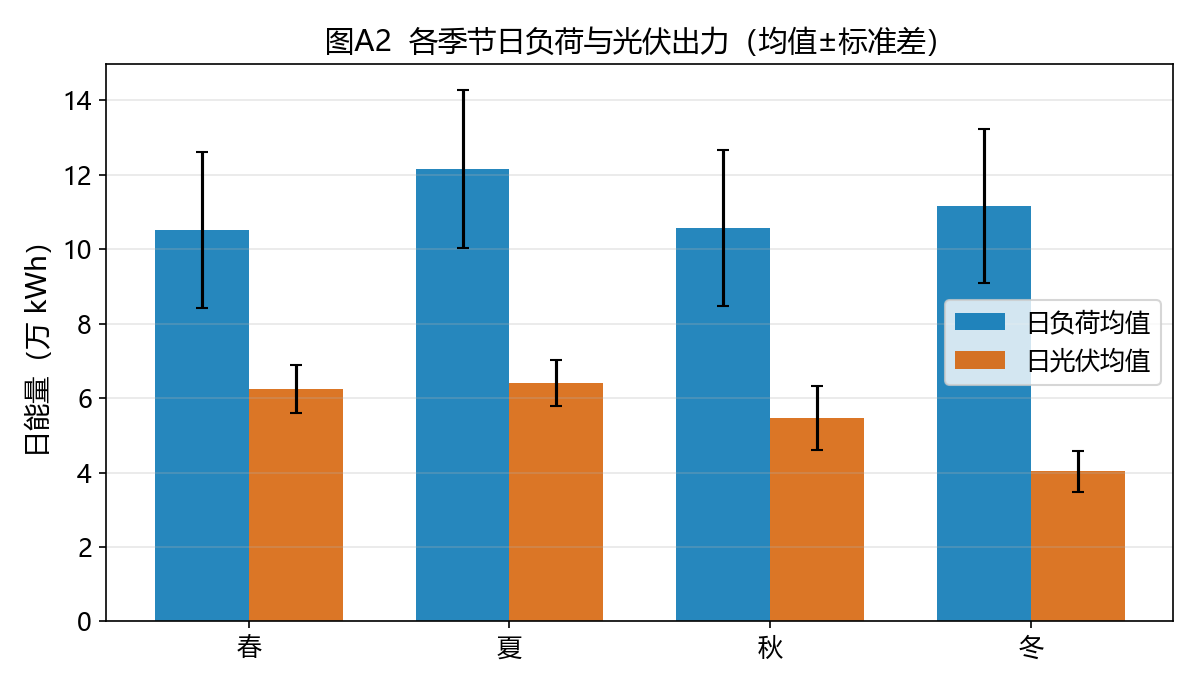
\includegraphics[width=0.8\textwidth]{figures_adv/A2_season_ld_pv.png}
    \caption{各季节日负荷与光伏出力（均值±标准差）}\label{fig:A2}
\end{figure}
在既有口径下计算各季节逐日购电费（图~\ref{fig:A1}），并统计附件 4 波动电价的
季节分布（图~\ref{fig:A3}），单因素方差分析表明季节间购电费差异高度显著（F=28.7，
$p=1.17\times10^{-16}$）：
\begin{table}[H]
    \centering
    \caption{季节统计：负荷、光伏、电价与购电费}\label{tab:season}
    \begin{tabular}{lccccc}
        \toprule[0.8pt]
        季节 & 日负荷/kWh & 日光伏/kWh & 日电价/(元/$\cdot$kWh) & 日购电费/元 & 峰谷比 \\
        \midrule[0.5pt]
        春 & 105200 & 62474 & 0.705 & 40300 & 2.11 \\
        夏 & 121530 & 64151 & 0.795 & 52000 & 1.97 \\
        秋 & 105749 & 54634 & 0.734 & 46700 & 2.11 \\
        冬 & 111574 & 40335 & 0.832 & 61100 & 2.30 \\
        \bottomrule[0.8pt]
    \end{tabular}
\end{table}
\begin{figure}[H]
    \centering
    \begin{minipage}[t]{0.48\textwidth}
        \centering
        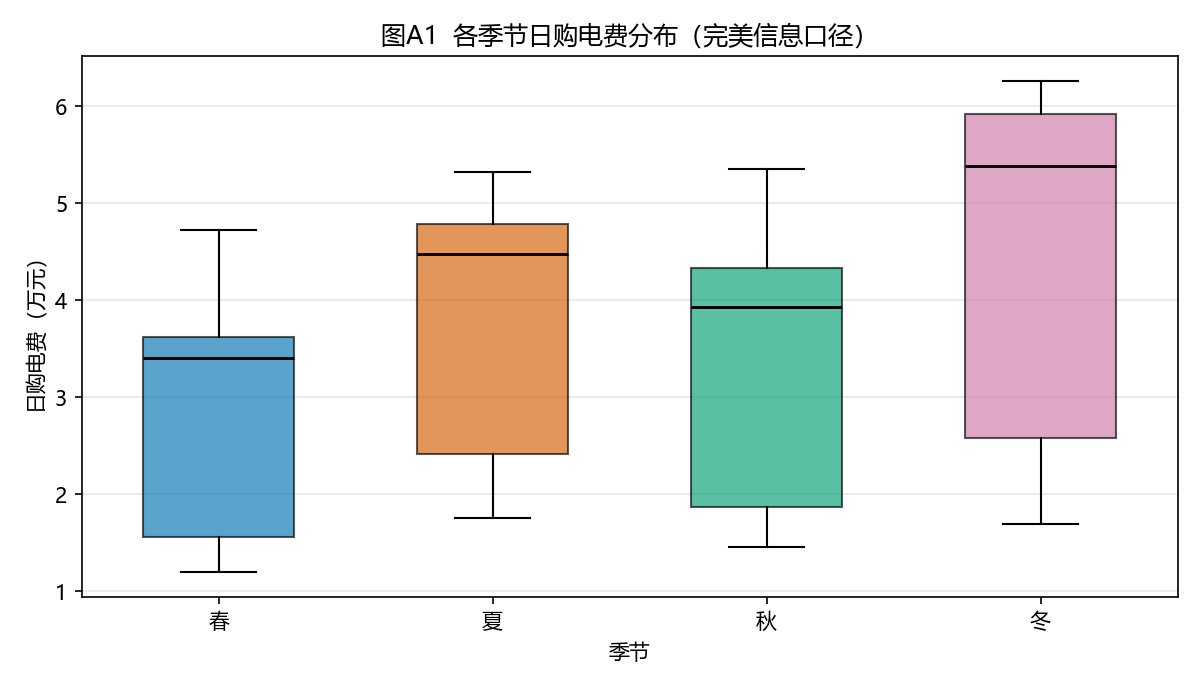
\includegraphics[width=\textwidth]{figures_adv/A1_season_cost_box.png}
        \caption{各季节日购电费分布}\label{fig:A1}
    \end{minipage}\hfill
    \begin{minipage}[t]{0.48\textwidth}
        \centering
        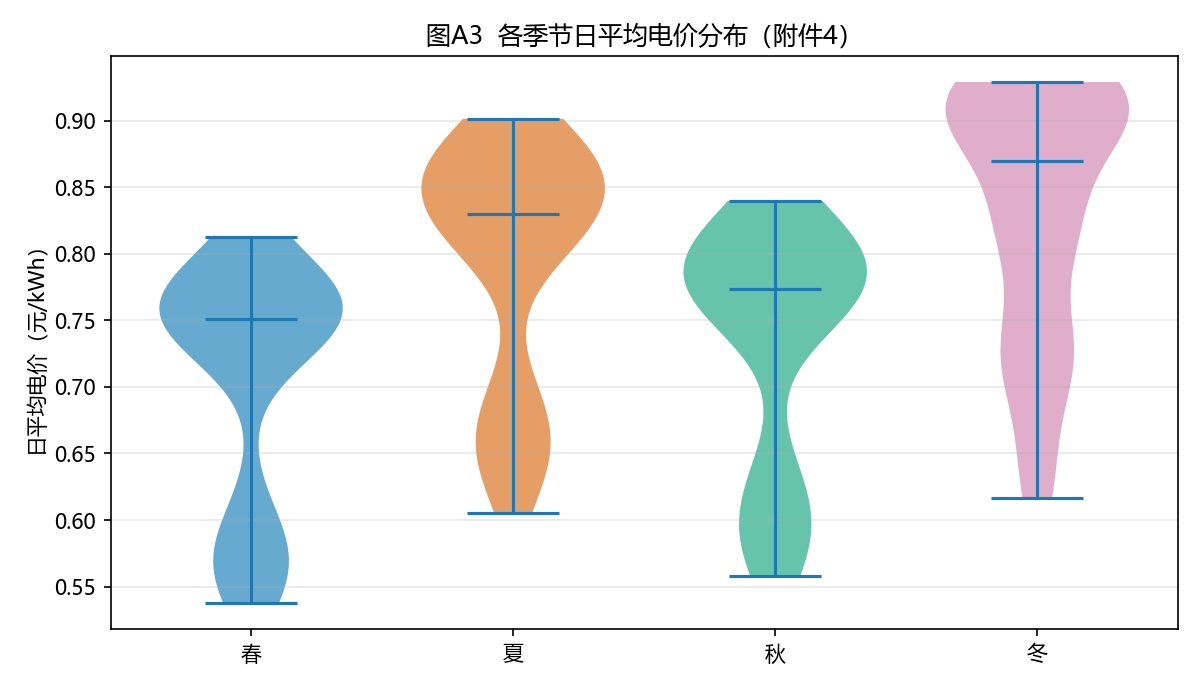
\includegraphics[width=\textwidth]{figures_adv/A3_price_violin.png}
        \caption{各季节日平均电价分布（附件 4）}\label{fig:A3}
    \end{minipage}
\end{figure}
冬季购电费为春季的 $1.56$ 倍，其机理是"光伏最低 + 电价最高 + 负荷峰谷差最大"三重叠加。
据此，在问题二的情景生成中按季节截取历史窗，并在问题四中按季节拆分解读电价波动风险。

\subsection{紧急情况统计与供电可靠性定位}
微网运行中，"紧急缺电"并非偶发的边缘情形，而是必须正面克服的现实威胁。为了论证本文以\textbf{供
电可靠性为主、经济性为辅}的优化目标，先对全年的紧急情况做定量统计。

\textbf{紧急情况的定义。}以决策日 0:00 可获得的预报信息为准（严格信息因果），定义当日净需求
$n_d=\sum_t(D_t-G_t)$，其 0:00 点预报 $\hat n_d$ 由负荷前 $K_{\mathrm{L}}=15$ 日逐时段均值与
附件 3 光伏 0:00 预报求得。日净需求预报偏差
\begin{equation}
    \varepsilon_d \;=\; \frac{n_d-\hat n_d}{\hat n_d},
    \label{eq:eps}
\end{equation}
$\varepsilon_d>0$ 表示实际净需求被低估、存在缺电风险。参照工程经验，取\textbf{低估超过 $20\%$
记为紧急波动日}。

\textbf{全年统计。}对 2025 年全年 365 天逐日统计（图~\ref{fig:emerg_series}）：低估 $\ge20\%$
的紧急波动日共 $156$ 天（$42.7\%$），低估 $\ge30\%$ 的仍有 $63$ 天（$17.3\%$），说明大幅低估
并非小概率事件。阈值敏感性检验表明，若把阈值放宽到 $10\%$ 则达 $235$ 天（$64.4\%$）、收紧到
$30\%$ 仍有 $63$ 天，$20\%$ 的取值在"不过度敏感、又不遗漏风险"之间。与之对应，全年实际触发
紧急购电的天数为 $166$ 天，其中"低估 $\ge20\%$ 且触发紧急购电"的严重缺电日 $109$ 天、单日紧急
购电超过 $50$~kWh 的有 $100$ 天，全年紧急购电合计 $148180$~kWh。按季节拆分（图~\ref{fig:emerg_season}），
春、夏两季紧急波动日最多（各约 $47\sim48$ 天，占各季 $51\%\sim52\%$），秋季 $37$ 天、冬季 $24$ 天；
冬季虽紧急波动日占比最低，但叠加全年最低的光伏出力与最高电价，一旦低估缺电，其购电费用冲击最大，
这也与图~\ref{fig:A1} 冬季购电费最高（$61100$~元/日）相互印证。
\begin{figure}[H]
    \centering
    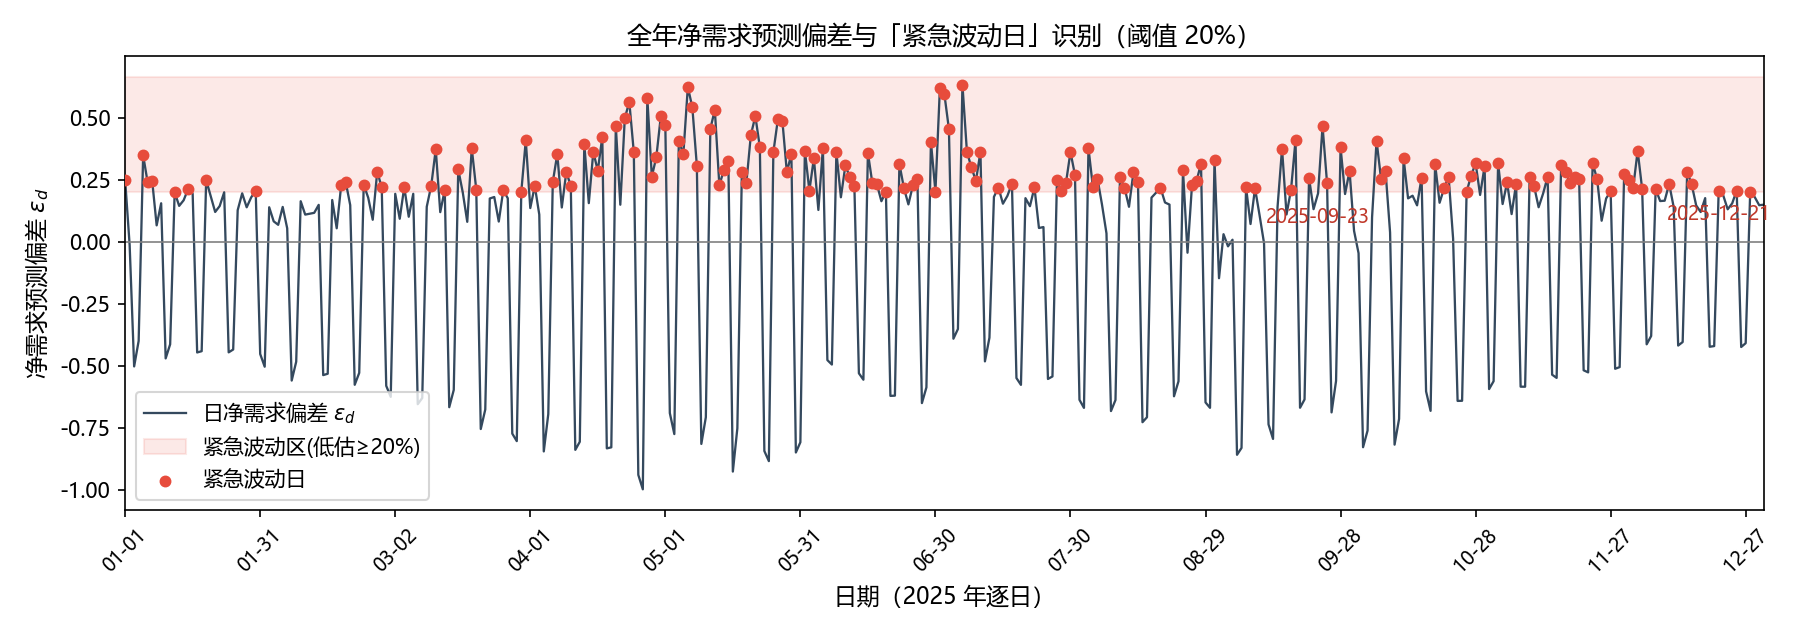
\includegraphics[width=0.92\textwidth]{figures_adv/emergency_series.png}
    \caption{全年日净需求预报偏差 $\varepsilon_d$ 序列与 $20\%$ 紧急波动带（红点为紧急波动日）}
    \label{fig:emerg_series}
\end{figure}
\begin{figure}[H]
    \centering
    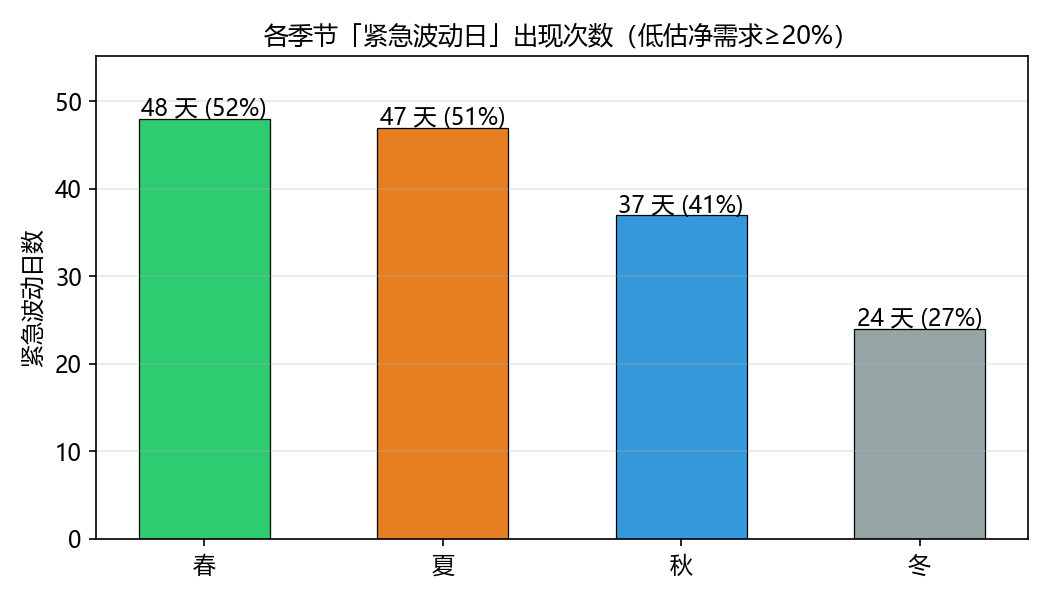
\includegraphics[width=0.7\textwidth]{figures_adv/emergency_season.png}
    \caption{各季节紧急波动日次数与占比}\label{fig:emerg_season}
\end{figure}
上述统计表明，净需求低估 $\ge20\%$ 的日期占比超过四成，紧急缺电是高频、季节聚集的现实威胁，
一旦发生将以 5 倍电价兜底并可能造成供电中断。因此本文把\textbf{供电可靠性置于经济性之前}：后文
问题二以 CVaR 风险项主动增加计划购电、压低紧急缺电的尾部损失，问题三以滚动再计划在预报更新时
及时削减紧急购电，均以可控的费用代价换取供电稳定性，而非单纯追求购电费用最低。

综合上述分析，本文的问题分析可抽象为"输入数据 $\to$ 统一建模内核 $\to$ 四子问题递进 $\to$
结果输出与校验"的总体流程。各子问题的区别仅在于\textbf{不确定性刻画颗粒度、决策信息结构与价
格冲击}，而同源共享功率—能量守恒内核与"计划—调整—紧急"三层购电结构。

\section{模型假设}
\begin{enumerate}
    \item 每个时段（10 分钟）内电价、负荷、光伏出力与购电量视为恒定；
    \item 功率与能量以时段换算，能量 = 功率 $\times 1/6$ h，充放电效率固定为 $90\%$，
          且充、放电不同时进行；
    \item 储能容量在 $1200\sim10800$~kWh 内运行，即时功率不超过 $5000$~kW；
    \item 问题二“完美信息口径”：因附件 2 给出全年实际数据，建模时假设能量在每天 0:00
          已知当日实际负荷与光伏（回顾性口径），故完美信息下无需紧急购电；其不确定性影响
          通过方法层的两阶段随机规划另行评估；
    \item 问题三只利用题目给定时刻（0/6/12/18）的整点光伏预报，负荷视为已知；
    \item 紧急购电、计划购电、调整购电均以外网无限供应为前提，不设购电上限。
\end{enumerate}

\section{符号说明}
为便于阅读，将正文使用的统一符号在一张三线表中逐行列出。符号严格对应赛题口径，
单时段时长为 $1/6$~h，能量量纲以 kWh 计。
\begin{center}
    \renewcommand{\arraystretch}{1.3}
\end{center}
\begin{longtable}{clc}
    \caption{主要符号说明}\label{tab:symbol}\\
    \toprule[0.8pt]
    \textbf{符号} & \textbf{符号说明} & \textbf{单位} \\
    \midrule[0.5pt]
    \endfirsthead
    \multicolumn{3}{l}{\bfseries 续上表}\\[-4pt]
    \midrule[0.5pt]
    \endhead
    \multicolumn{3}{l}{（续表下页）}\\
    \bottomrule[0.8pt]
    \endfoot
        $T,\ t$ & 每日时段数与时段下标 ($T=144$) & -- \\
        $P_t$ & 时段 $t$ 计划购电量（0:00 承诺） & kWh \\
        $A_t$ & 时段 $t$ 最终调整购电量 & kWh \\
        $Q_t$ & 时段 $t$ 紧急购电量 & kWh \\
        $u_t,\,w_t$ & 时段 $t$ 违约量 / 超购量 & kWh \\
        $G_t$ & 时段 $t$ 光伏出力 & kWh \\
        $D_t$ & 时段 $t$ 小区负荷 & kWh \\
        $R_t$ & 时段 $t$ 弃光电量 & kWh \\
        $E_t$ & 时段 $t$ 末储电量 & kWh \\
        $E_0$ & 日初储电量 ($=6000$) & kWh \\
        $c_t,\,f_t$ & 时段 $t$ 充电量 / 放电量 & kWh \\
        $\eta$ & 充放电效率 ($=0.9$) & -- \\
        $E_{\min},E_{\max}$ & 储能运行上下界 ($1200,\ 10800$) & kWh \\
        $\bar{E}$ & 单时段最大充/放能量 ($=5000/6$) & kWh \\
        $S,\ s$ & 情景总数 / 情景下标 & -- \\
        $\hat G^s,\hat D^s$ & 第 $s$ 情景的光伏 / 负荷实现 & kWh \\
        $G_t^{(\tau)}$ & $\tau$ 时点对时段 $t$ 的光伏预报 & kWh \\
        $\tau$ & 滚动决策时点（取 $0,6,12,18$） & h \\
        $\psi^s$ & 第 $s$ 情景总成本 & 元 \\
        $\alpha$ & CVaR 中的 VaR 值（自由变量） & 元 \\
        $z_s$ & 第 $s$ 情景超额损失 ($z_s\ge\psi^s-\alpha$) & 元 \\
        $p_t$ & 时段 $t$ 电价（附件 1） & 元/kWh \\
        $p_t^{var}$ & 时段 $t$ 波动电价（附件 4） & 元/kWh \\
        $\lambda$ & CVaR 风险厌恶权重 & -- \\
        $\beta$ & CVaR 置信水平 ($=0.9$) & -- \\
        $k$ & 季节下标（春/夏/秋/冬） & -- \\
        \bottomrule[0.8pt]
    \end{longtable}

\section{模型建立与求解}

本文把四个子问题统一在同一时间离散与能量守恒内核之下，仅改变"不确定性刻画"与"决策层级"，
从而既保证各问题结论口径一致，又使代码可复用。为此，首先明确\textbf{决策变量在时序与信息结
构上的区分}：所谓"计划购电 $P_t$"是每天 0:00 承诺的某时段购电量，作为一阶段决策对各情景/各日
共用；问题三在后续时点引入"调整购电 $A_t$"，是对计划的修正；而 "紧急购电 $Q_t$"仅在日终对
实际出力短缺作事后兜底，价格高达 5 倍。三者共同构成本文贯穿全篇的\textbf{"计划—调整—紧急"
三层购电结构}，也是后续各问题建模的公共骨架。

以每天 0:00 储电量 $E_0$ 出发，任意一天的功率-能量守恒为：
\begin{equation}
    P_t + G_t + \eta f_t + Q_t \;=\; D_t + c_t + R_t,\qquad t=1,\ldots,T
    \label{eq:balance}
\end{equation}
式~\eqref{eq:balance} 表明：购电、光伏、放电、紧急购电之和 = 负荷、充电、弃光之和；等式左端
为微网"供应"侧，右端为"消纳"侧，二者在每个时段必须严格相等，故式~\eqref{eq:balance} 亦称
微网功率平衡约束。值得强调的是，式~\eqref{eq:balance} 中光伏放电合流、弃光 $R_t$ 作为非负
松弛变量出现，意味着若某时段光伏过剩可主动弃光，从而允许"供大于需"，避免强行充电超出储能上限。
储能递推与约束为：
\begin{align}
    E_t &= E_{t-1} + \eta c_t - f_t, \label{eq:soc}\\
    E_{\min} &\le E_t \le E_{\max}, \quad 0\le c_t,f_t \le \bar{E}, \label{eq:socbound}
\end{align}
其中 $\bar{E}=5000/6$~kWh 为单时段最大充/放能量（由功率上限换算）。式~\eqref{eq:soc} 是能量
在时间的转移方程：充电使储能增加（效率 $\eta=0.9$），放电使其减少；由于 $\eta\le1$，时际间会
存在不可避免的能量损耗，这使得系统在能量维度上具有"不可逆性"，也是储能参与经济调度的价值源泉
——它允许用当下的低价电能置换未来的高价电能。式~\eqref{eq:socbound} 同时限定了储能运行区间
与单时段的充放功率，防止越限造成设备损坏，并隐含约定充放不可同时进行。

\subsection{问题一：确定性每日计划（LP）}
\begin{figure}[H]
    \centering
    \begin{tikzpicture}[node distance=0.5cm and 0.5cm]
        \node[flbox] (a1) {读取附件全年数据};
        \node[flbox, right=of a1] (a2) {日期对齐与校验};
        \node[flbox, right=of a2] (a3) {构建目标函数};
        \node[flbox, below=of a3] (b3) {储能日循环约束};
        \node[flbox, left=of b3] (b2) {逐日独立 LP 优化};
        \node[flbox, left=of b2] (b1) {汇总全年购电结果};
        \node[flbox, below=of b1] (c1) {输出指定时段计划};
        \node[flbox, right=of c1] (c2) {能量守恒校验};
        \node[flbox, right=of c2] (c3) {结果检验分析};
        \draw[flarr] (a1) -- (a2); \draw[flarr] (a2) -- (a3);
        \draw[flarr] (a3) -- (b3); \draw[flarr] (b3) -- (b2);
        \draw[flarr] (b2) -- (b1); \draw[flarr] (b1) -- (c1);
        \draw[flarr] (c1) -- (c2); \draw[flarr] (c2) -- (c3);
    \end{tikzpicture}
    \caption{问题一求解流程图}\label{fig:flowq1}
\end{figure}
问题一采用``逐日独立求解''的确定性路线：全年 365 天逐日建立 LP 并由 HiGHS 求全局最优，
整体求解流程如图~\ref{fig:flowq1} 所示。

\subsubsection{线性规划模型的建立}
针对问题一"电价、负荷与光伏预测均已知"的完美信息场景，以每天 10 分钟为一个时段
（$T=144$），决策变量为各时段计划购电量 $P_t$、充电量 $c_t$、放电量 $f_t$、弃光量 $R_t$
与各时段末储电量 $E_t$。由于信息完备且无缺电风险，紧急购电 $Q_t\equiv0$。目标为最小化当日
购电费用：
\begin{equation}
    \min \ \sum_{t=1}^{T} p_t\, P_t
    \label{eq:obj1}
\end{equation}
\textbf{s.t.}
\begin{subequations}\label{eq:lp1}
\begin{alignat}{2}
    & P_t + G_t + \eta f_t + Q_t \;=\; D_t + c_t + R_t, && t=1,\ldots,T \label{eq:lp1a}\\
    & E_t \;=\; E_{t-1} + \eta c_t - f_t, && t=1,\ldots,T \label{eq:lp1b}\\
    & E_{\min} \le E_t \le E_{\max}, && t=1,\ldots,T \label{eq:lp1c}\\
    & 0\le c_t\le \bar{E},\quad 0\le f_t\le \bar{E}, && t=1,\ldots,T \label{eq:lp1d}\\
    & E_T = E_0 = 6000, && t=T \label{eq:lp1e}\\
    & P_t\ge0,\ R_t\ge0,\ Q_t=0,\ \forall t. \label{eq:lp1f}
\end{alignat}
\end{subequations}
约束式~\eqref{eq:lp1a} 为微网逐时段功率-能量守恒（对应题目"微网提供的电能不低于小区负载
""及"可弃光"的设定）：左端为微网供应侧（购电、光伏、放电、紧急购电），右端为消纳侧
（负荷、充电、弃光），弃光 $R_t$ 作为非负松弛变量，允许光伏过剩时主动弃光；
式~\eqref{eq:lp1b} 为储能能量递推（题目给定储能充放电效率 $\eta=0.9$，充电使储电增加、放电
使之减少）；式~\eqref{eq:lp1c} 为储能容量约束（题目：运行区间 $1200\sim10800$~kWh）；
式~\eqref{eq:lp1d} 为单时段充放电功率上限（题目：即时功率上限 $5000$~kW，即单时段最大
$\bar{E}=5000/6$~kWh，并隐含充放不可同时超过该上限）；式~\eqref{eq:lp1e} 为储能"日循环"
约束（题目要求 0:00 与 24:00 储电量相同，$E_0=6000$~kWh）；式~\eqref{eq:lp1f} 为变量非负
及问题一无紧急购电。\label{con:q1} 该问题为线性规划，用 $\verb|scipy.optimize.linprog|$
（HiGHS 求解器）逐日求全局最优\cite{rp:linprog}，全年 365 天求解流程如图~\ref{fig:flowq1}。

上述模型即为问题一的标准线性规划：目标函数（式~\eqref{eq:obj1}）最小化当日购电费，约束
（式~\eqref{eq:lp1a}--\eqref{eq:lp1f}）逐一对应题目给出的功率平衡、储能递推与容量、充放功率
上限、"日循环"与变量非负条件。由于信息完备，其最优解给出的购电费用 $35126.8$~元是后续各问题
在不确定性下的对照基准。

\subsubsection{结果分析}
\begin{table}[H]
    \centering
    \caption{问题一：指定时段购电量、全天汇总与充放电计划（kWh，购电费单位元）}\label{tab:q1}
    \begin{tabular}{cc|cc|cc}
        \toprule[0.8pt]
        指定时段 & 购电量 & 指定时段 & 购电量 & 指定时段 & 购电量 \\
        \midrule[0.5pt]
        10:00-10:10 & 0.0 & 12:00-12:10 & 486.4 & 14:00-14:10 & 0.0 \\
        16:00-16:10 & 394.9 & 18:00-18:10 & 637.0 & 20:00-20:10 & 0.0 \\
        \midrule
        全天购电量 & 59482.7 & 购电费（元） & 35126.8 & & \\
        \midrule
        时段 & 充电量 & 放电量 & 时段 & 充电量 & 放电量 \\
        \midrule[0.5pt]
        0:00-4:00 & 4500.0 & 0.0 & 4:00-8:00 & 833.3 & 6608.2 \\
        8:00-12:00 & 3954.6 & 2357.1 & 12:00-16:00 & 6119.4 & 101.2 \\
        16:00-20:00 & 0.0 & 5631.9 & 20:00-24:00 & 5333.3 & 3968.1 \\
        \midrule
        0:00 储电量 & 6000 & & 24:00 储电量 & 6000 & \\
        \bottomrule[0.8pt]
    \end{tabular}
\end{table}
由表~\ref{tab:q1}：白天光伏高发期（8:00--16:00）以充电为主，傍晚与凌晨
电价、负荷峰期以放电为主，储能在日末回到日初 $6000$~kWh，故日循环可持续。购电集中于电价
洼地，购电费最小为 $35126.8$~元。完整计划购电策略见 $result1.xlsx$，购电/充放电/储电轨迹如
图~\ref{fig:q1}。图~\ref{fig:sankey} 以 2025-06-21 为例给出微网能量流向，直观展示光伏供能、
储能充放与购电补缺的相对比例。
\begin{figure}[H]
    \centering
    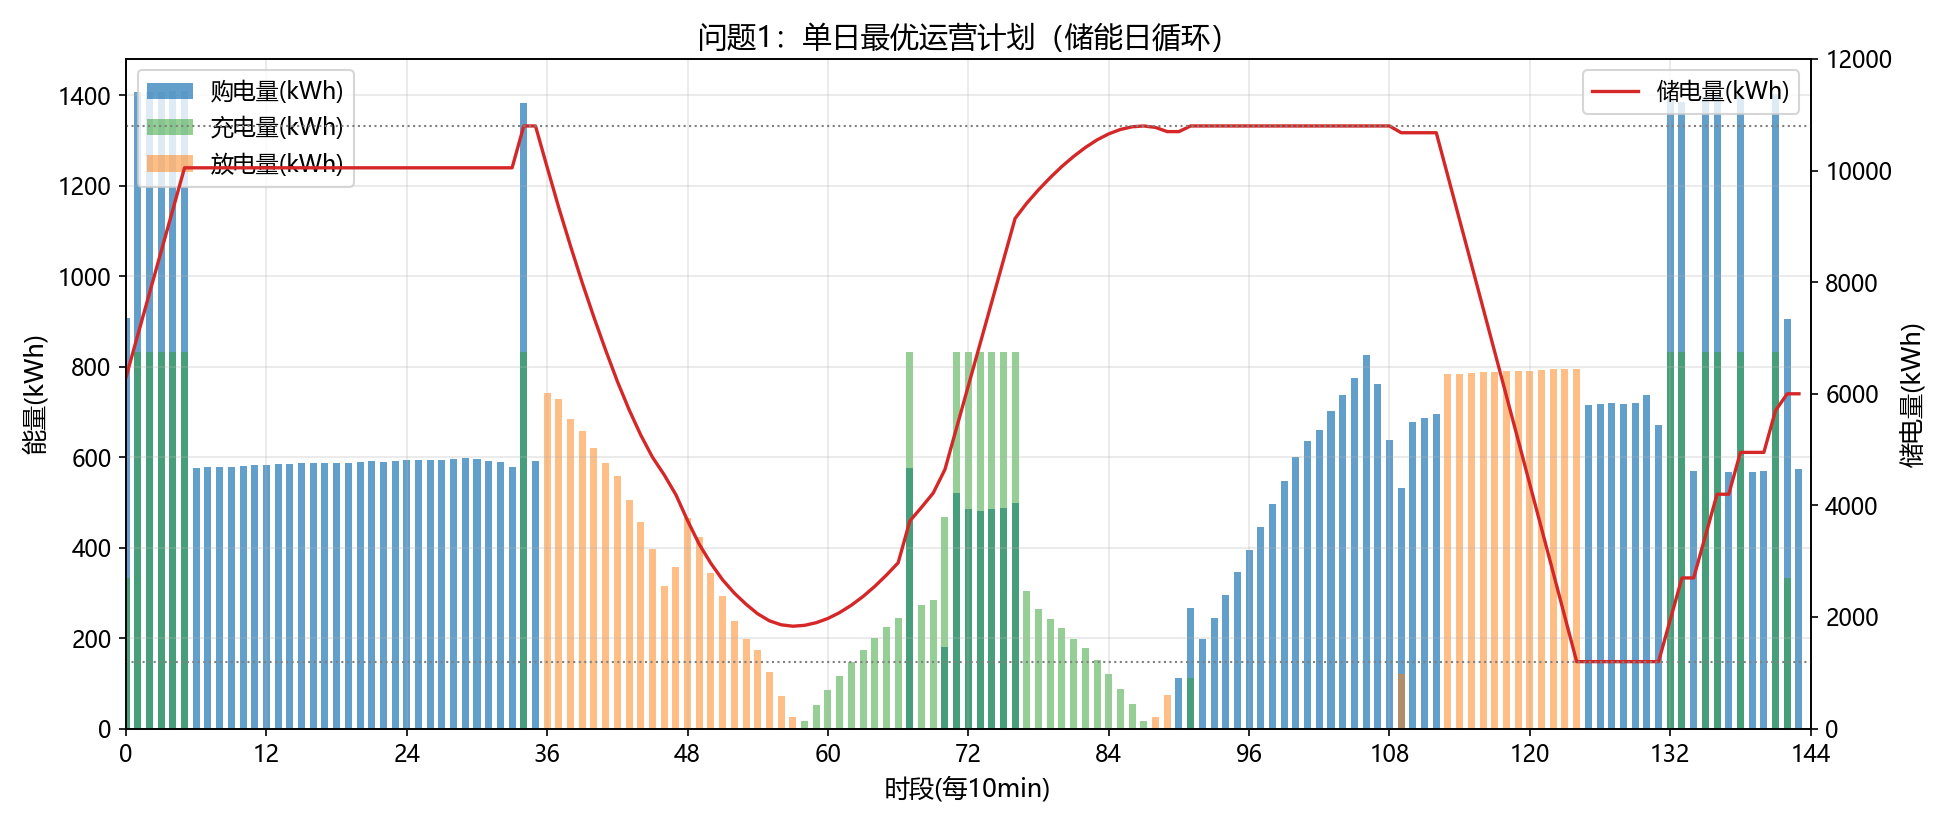
\includegraphics[width=0.95\textwidth]{figures/q1_plan.png}
    \caption{问题一：单日最优运营计划（储能日循环）}\label{fig:q1}
\end{figure}
\begin{figure}[H]
    \centering
    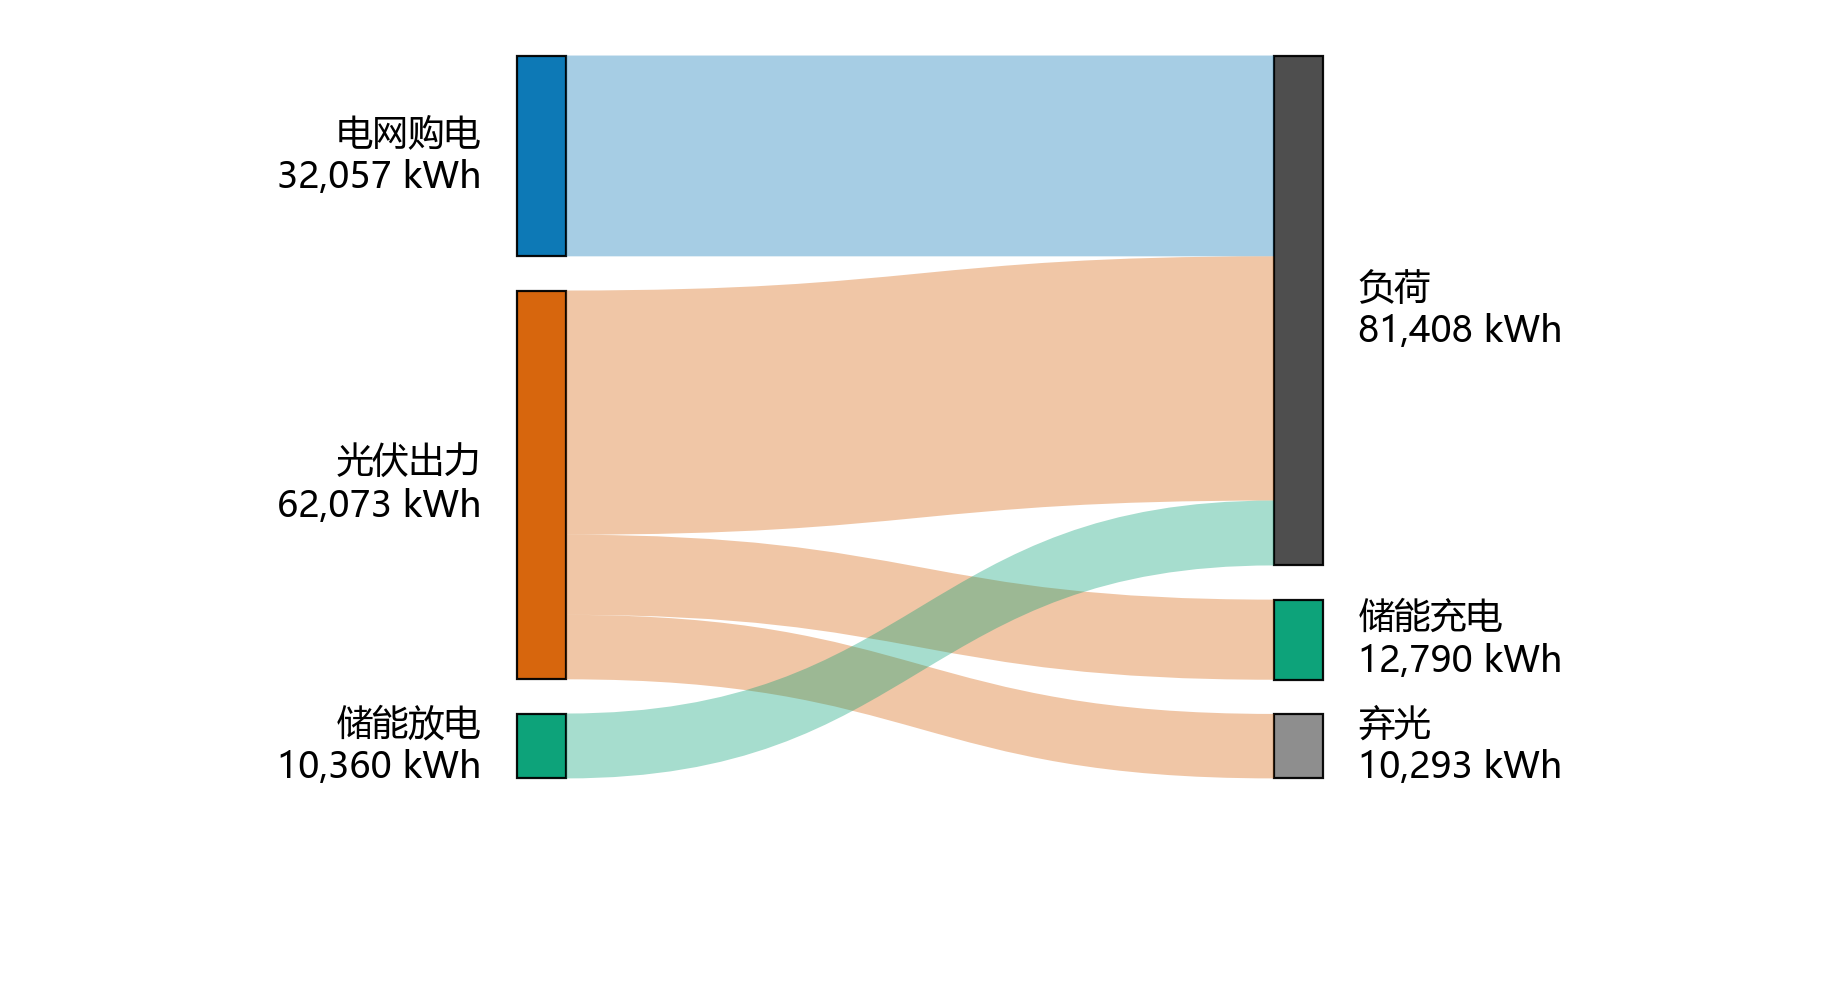
\includegraphics[width=0.82\textwidth]{figures_adv/A8_sankey.png}
    \caption{2025-06-21 微网能量流向桑基图（完美信息日）}\label{fig:sankey}
\end{figure}

\subsection{问题二：两阶段随机规划 + CVaR}
\begin{figure}[H]
    \centering
    \begin{tikzpicture}[node distance=0.5cm and 0.5cm]
        \node[flbox] (a1) {读取历史负荷/光伏};
        \node[flbox, right=of a1] (a2) {交叉验证选窗 $K$};
        \node[flbox, right=of a2] (a3) {残差 bootstrap 情景};
        \node[flbox, below=of a3] (b3) {两阶段随机规划};
        \node[flbox, left=of b3] (b2) {固定计划按实际结算};
        \node[flbox, left=of b2] (b1) {紧急购电 $Q$ 明细};
        \node[flbox, below=of b1] (c1) {输出四指定日结果};
        \node[flbox, right=of c1] (c2) {CVaR 参数敏感性};
        \node[flbox, right=of c2] (c3) {结果检验分析};
        \draw[flarr] (a1) -- (a2); \draw[flarr] (a2) -- (a3);
        \draw[flarr] (a3) -- (b3); \draw[flarr] (b3) -- (b2);
        \draw[flarr] (b2) -- (b1); \draw[flarr] (b1) -- (c1);
        \draw[flarr] (c1) -- (c2); \draw[flarr] (c2) -- (c3);
    \end{tikzpicture}
    \caption{问题二求解流程图}\label{fig:flowq2}
\end{figure}
问题二在 0:00 依据历史信息一次性形成全天计划，"预报—情景—优化—结算"链式流程
如图~\ref{fig:flowq2} 所示。

\subsubsection{随机规划模型的建立}
问题二在每天 0:00 制定计划时，并不知道当日实际的负荷与光伏出力（尽管题目给出了全年数据，但
决策时点只能使用截至前一日的滚动历史），因此这是一个不确定规划问题。本文采用\textbf{两阶段
随机规划}建模：设 $S$ 个等概率情景 $\{\hat G^s,\hat D^s\}_{s=1}^S$ 描述当日光伏与负荷的可能
实现（情景构造见下文）；第一阶段计划购电 $P_t$ 必须在任何情景实现之前作出，对各情景共用；第二
阶段按情景实现决定充放电量 $c^s_t,f^s_t$、紧急购电量 $Q^s_t$ 与弃光量 $R^s_t$。目标为最小化
计划购电费、期望紧急购电费与风险项之和：
\begin{equation}
    \min_{P}\ \sum_t p_t P_t \;+\; \frac1S \sum_{s=1}^S\sum_{t=1}^T 5 p_t Q_t^s
        \;+\; \lambda\, \mathrm{CVaR}_\beta\bigl(\psi^s\bigr),
    \label{eq:obj2}
\end{equation}
其中第 $s$ 个情景的总成本 $\psi^s=\sum_t\bigl(p_tP_t + 5p_t Q_t^s\bigr)$；前两项分别为计划购电
费与紧急购电费的期望值，末项 $\lambda\,\mathrm{CVaR}_\beta$ 是风险惩罚项，$\lambda$ 为风险厌恶
权重。

\textbf{关于 CVaR}。条件风险价值（Conditional Value at Risk，CVaR）是金融与电力领域中度量
"尾部风险"的常用指标：对随机损失 $\psi$，置信水平 $\beta$ 下的 $\mathrm{CVaR}_\beta$ 表示
最坏的 $100(1-\beta)\%$ 情景的平均损失，即"万一发生极端情景，平均要损失多少"。本文取
$\beta=0.9$，即关注最坏 $10\%$ 情景的平均购电成本。第二问之所以需要引入它，是因为若只最小化
期望费用（$\lambda=0$），模型会把极端缺电情景的高额紧急购电（5 倍电价）视为"小概率事件"而
掉以轻心，导致实际运行中偶发巨额的紧急购电费用；而 $\lambda>0$ 时，模型会有意多预留一些计划
购电，把极端情景的尾部损失压下来。风险厌恶权重 $\lambda$ 越大，计划购电越保守，紧急购电量越少
（见第 5.2.3 节的权衡分析），$\lambda=0$ 则退化为纯期望费用最小化。CVaR 可改写为如下线性约束
\cite{rp:cvar,cn:cvar}：
\begin{equation}
    \mathrm{CVaR}_\beta \;=\; \alpha + \frac{1}{(1-\beta)S}\sum_{s=1}^S z_s,
    \qquad z_s\ge \psi^s-\alpha,\quad z_s\ge0,
    \label{eq:cvar}
\end{equation}
其中 $\alpha$ 为自由变量（对应 VaR，即最坏情景的分位点），$z_s$ 为第 $s$ 个情景超出 $\alpha$
的超额损失；如此非光滑的风险项即化为线性不等式，整个模型仍是一个可全局求解的线性规划
\cite{cn:stoch}。

\textbf{s.t.} 对每个情景 $s=1,\ldots,S$，约束为：
\begin{subequations}\label{eq:lp2}
\begin{alignat}{2}
    & P_t + G_t^s + \eta f_t^s + Q_t^s \;=\; D_t^s + c_t^s + R_t^s, && t=1,\ldots,T \label{eq:lp2a}\\
    & E_t^s \;=\; E_{t-1}^s + \eta c_t^s - f_t^s, && t=1,\ldots,T \label{eq:lp2b}\\
    & E_{\min} \le E_t^s \le E_{\max}, && t=1,\ldots,T \label{eq:lp2c}\\
    & 0\le c_t^s\le \bar{E},\quad 0\le f_t^s\le \bar{E}, && t=1,\ldots,T \label{eq:lp2d}\\
    & z_s \ge \psi^s - \alpha,\quad z_s \ge 0, && s=1,\ldots,S \label{eq:lp2e}\\
    & P_t\ge0,\ Q_t^s\ge0,\ R_t^s\ge0, && \forall s,t \label{eq:lp2f}
\end{alignat}
\end{subequations}
式~\eqref{eq:lp2a} 为各情景下的功率-能量守恒（同问题一）；式~\eqref{eq:lp2b}--\eqref{eq:lp2d}
为储能递推与容量、功率约束；式~\eqref{eq:lp2e} 为 CVaR 线性化；式~\eqref{eq:lp2f} 为变量
非负。计划购电 $P_t$ 不带情景上标，即"非预期性"（non-anticipativity）——0:00 的决策不能利用
任何未来信息。

\subsubsection{预测与情景生成}
情景与点预报构造坚持\textbf{信息因果}原则：每日 0:00 只使用当天之前的历史数据。点预报取
负荷、光伏各自前 $K_{\text{L}}/K_{\text{P}}$ 天逐时段（144）的均值，$K$ 通过全年（2.1--12.31）
逐日交叉验证、按归一化 RMSE 选取。为排除从稀疏候选集取点带来的偶然性，本文将窗口 $K$ 在
$\{1,\ldots,40\}$ 上做细粒度扫描（图~\ref{fig:Ksens}）：负荷的归一化 RMSE 在 $K\in[8,16]$
呈浅谷、$K=15$ 落在谷底附近，而 $K=1$ 仅为无历史平滑的单日冷启动伪最优（物理上不可靠）；光伏
的归一化 RMSE 在 $K\in[5,7]$ 呈接近水平的平坦平台（差异 $<5\times 10^{-4}$），取整数周周期
$K=7$ 兼具最小化与可解释性。据此选定 $K_{\text{L}}=15,\ K_{\text{P}}=7$，并在后续以点预报为
"居中基准"叠加残差情景，故 $K$ 的微小扰动对全年费用影响甚微（敏感性分析见第 6.3 节），论证了
$K$ 选取的稳健性；
\begin{figure}[H]
    \centering
    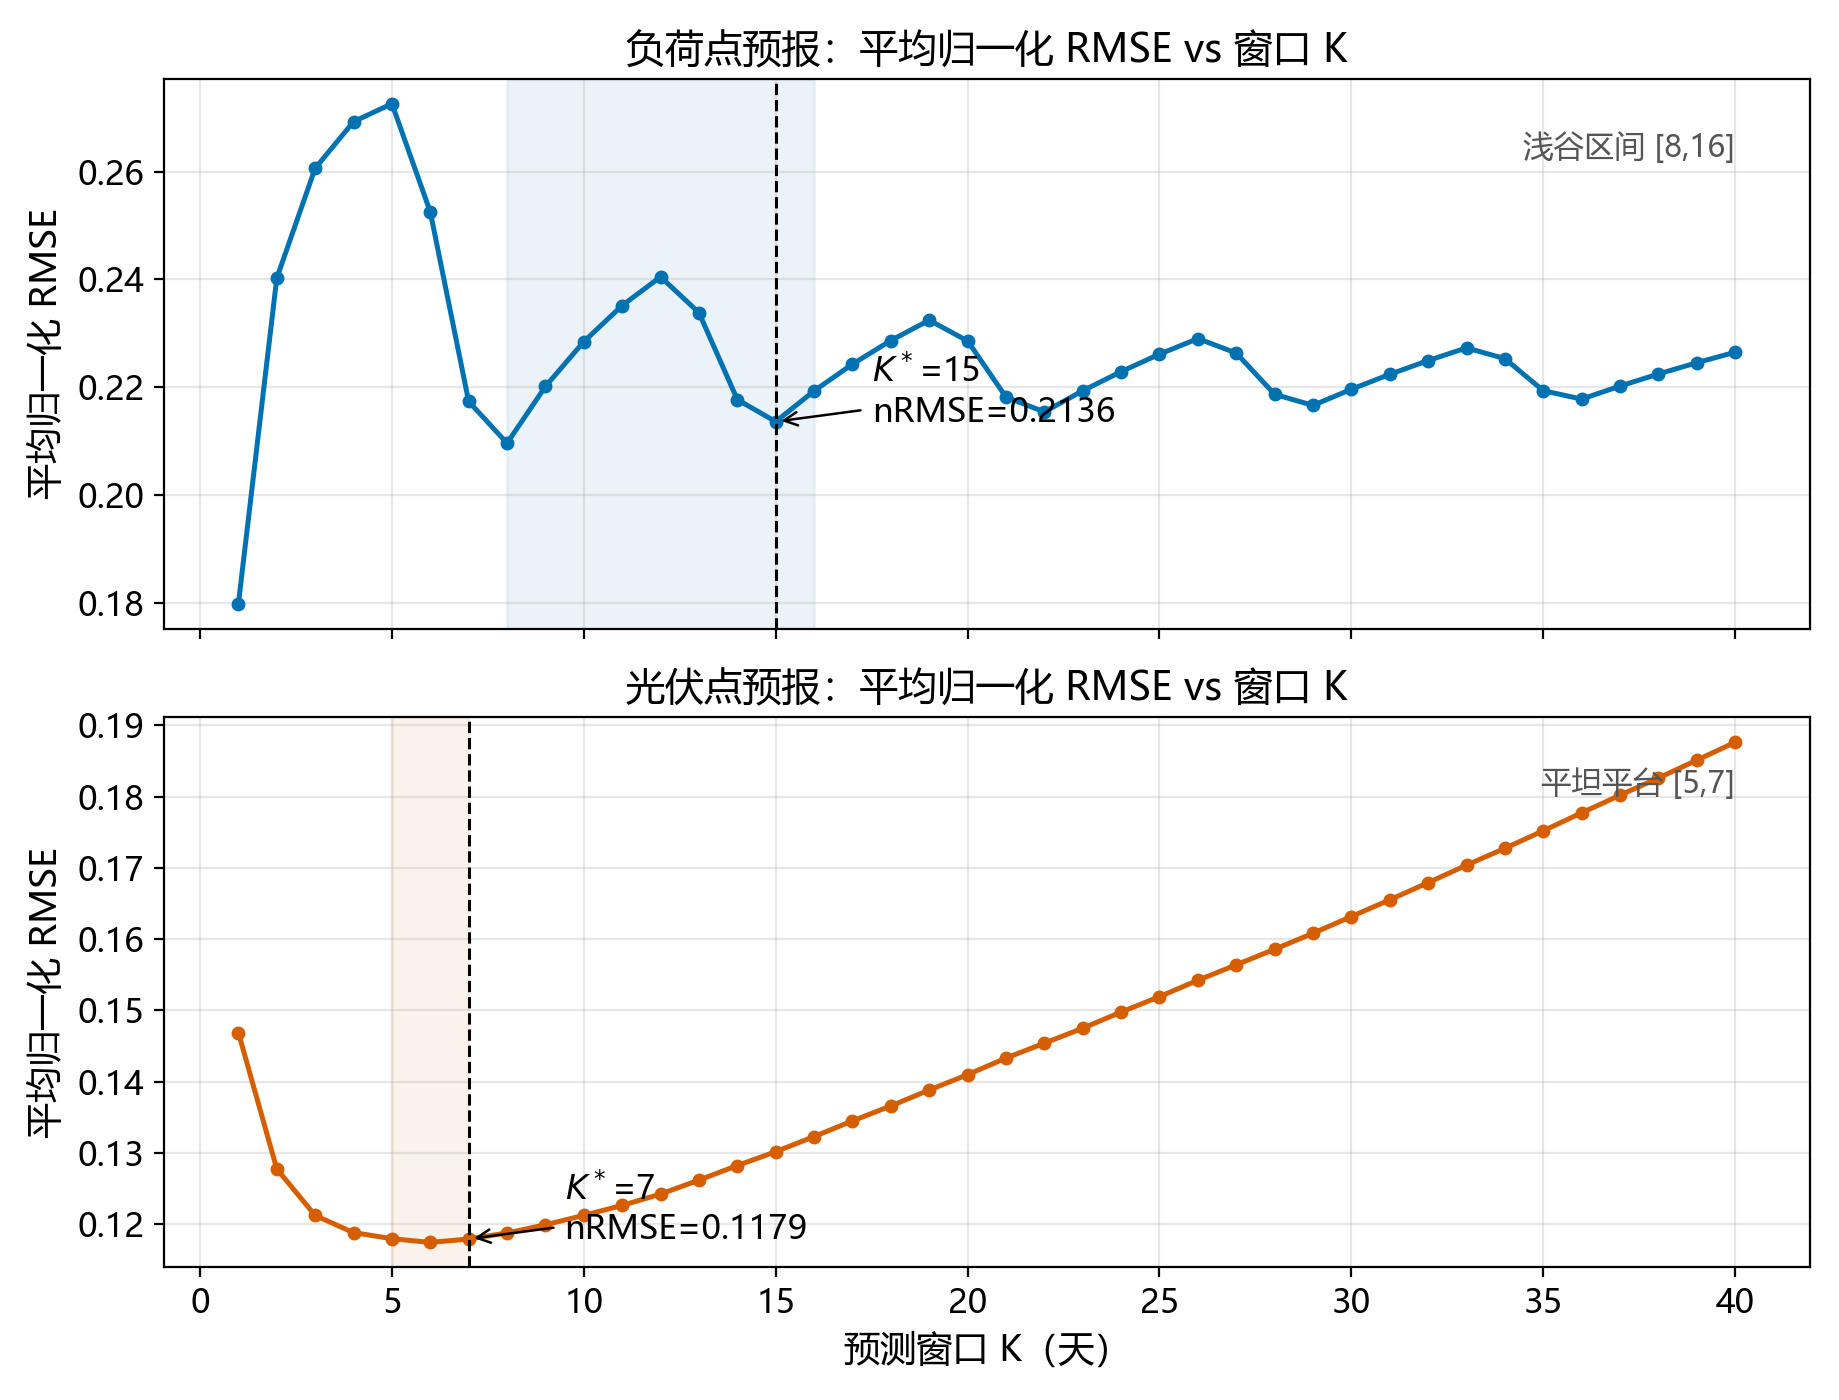
\includegraphics[width=0.9\textwidth]{figures_adv/q2_K_sensitivity.png}
    \caption{点预报窗口 $K$ 的全年交叉验证敏感性（上：负荷，下：光伏）}\label{fig:Ksens}
\end{figure}
情景则采用\textbf{整日成对残差 bootstrap}：先按最长时间窗取最近 $w$ 天历史，逐槽计算
"实际$\ -$点预报"的整日残差，再有放回抽取 $S=30$ 个整天（负荷与光伏同一天成对取样，从而保留
两者相关性），情景 = 点预报 + 抽取的整日残差，光伏截断到非负。2025-01-01 缺乏历史，以附件 1
典型日剖面作冷启动基准。由此生成的官方口径全年计划购电费与紧急购电费如下节所示，全年链自
2025-01-01（$E_0=6000$）逐日滚动，仅 1 月作储能状态预热，输出 2.1--12.31。

\subsubsection{结果分析}
在上述预报式口径下，以 $S=30$ 情景做两阶段随机规划得计划购电 $P$，再以当日实际负荷/光伏
结算得紧急购电 $Q$，全年（2.1--12.31）计划购电费 $15726290.4$~元、紧急购电费
$478538.6$~元（紧急购电 $148180$~kWh），合计 $16204829.0$~元。表~\ref{tab:q2} 给出四个
指定日期的结果（完整见 $result2.xlsx$）。
\begin{table}[H]
    \centering
    \caption{问题二：预报式两阶段随机规划指定日期结果（单位 kWh、元）}\label{tab:q2}
    \begin{tabular}{ccccc}
        \toprule[0.8pt]
        日期 & 计划购电费 & 紧急购电量 & 紧急购电费 & 24:00 储电量 \\
        \midrule[0.5pt]
        2025-03-20 & 43652.3 & 29.3 & 197.4 & 1200 \\
        2025-06-21 & 49345.5 & 0 & 0 & 1200 \\
        2025-09-23 & 40734.3 & 1666.5 & 5526.6 & 1200 \\
        2025-12-21 & 60328.7 & 148.5 & 501.5 & 1200 \\
        \bottomrule[0.8pt]
    \end{tabular}
\end{table}
\noindent\textit{注：}表~\ref{tab:q2} 计划购电费为两阶段随机规划的一阶段计划购电在当日实际
电价下的费用；6-21 为周末，负荷低于工作日，当日实际净需求低于全部情景包络，计划与储能即可
完全吸收缺电，故紧急购电为 0（而非观测缺仓）；24:00 储电量趋向运行下界 $1200$~kWh，属低谷
电价时段释放电能的补电行为。全年各日 144 时段逐时段紧急购电见 $result2.xlsx$。

\subsubsection{CVaR 风险评估与权衡方法}
为回答"当决策者愿意以少量计划费用换取供电可靠性时，应如何权衡"，本文在目标函数
式~\eqref{eq:obj2} 中引入风险权重 $\lambda$ 的 CVaR 尾部项，并先对全年（2.1--12.31）
逐 $\lambda\in\{0,0.5,1,2,5\}$ 整链重跑（各 $\lambda$ 自 2025-01-01、$E_0=6000$ 独立滚动，
1 月仅作储能预热），得到全年"计划费—紧急费—总费"随 $\lambda$ 的演化
（$report/q2\_lambda\_year\_scan.csv$）。结果表明：$\lambda$ 从 0 增至 0.5，计划购电费仅上浮
$3.9\%$（$15133792.3\to15726290.4$~元），而紧急购电费削减 $55.5\%$（$1074587.3\to478538.6$~元），
全年合计费用基本持平（$16208379.6\to16204829.0$~元，$-0.02\%$）。据此按"紧急费降至 $\lambda=0$
的 $60\%$ 以内且总费上浮不超过 $1\%$"的数据驱动准则选定官方口径 $\lambda^*=0.5$，使全年结果在
几乎不增加总成本的前提下把缺电风险的显式成本削减过半。
为刻画单日粒度上的风险—费用折中，针对四个指定日期逐一求解 $\lambda\in\{0,0.5,1,2,5\}$，
以其计划购电费 $P$ 对当日实际负荷/光伏结算，得到随 $\lambda$ 演化的计划费—紧急费折中关系，
其帕累托前沿见图~\ref{fig:pareto}，参数稳健性见第 6.2 节。
\begin{figure}[H]
    \centering
    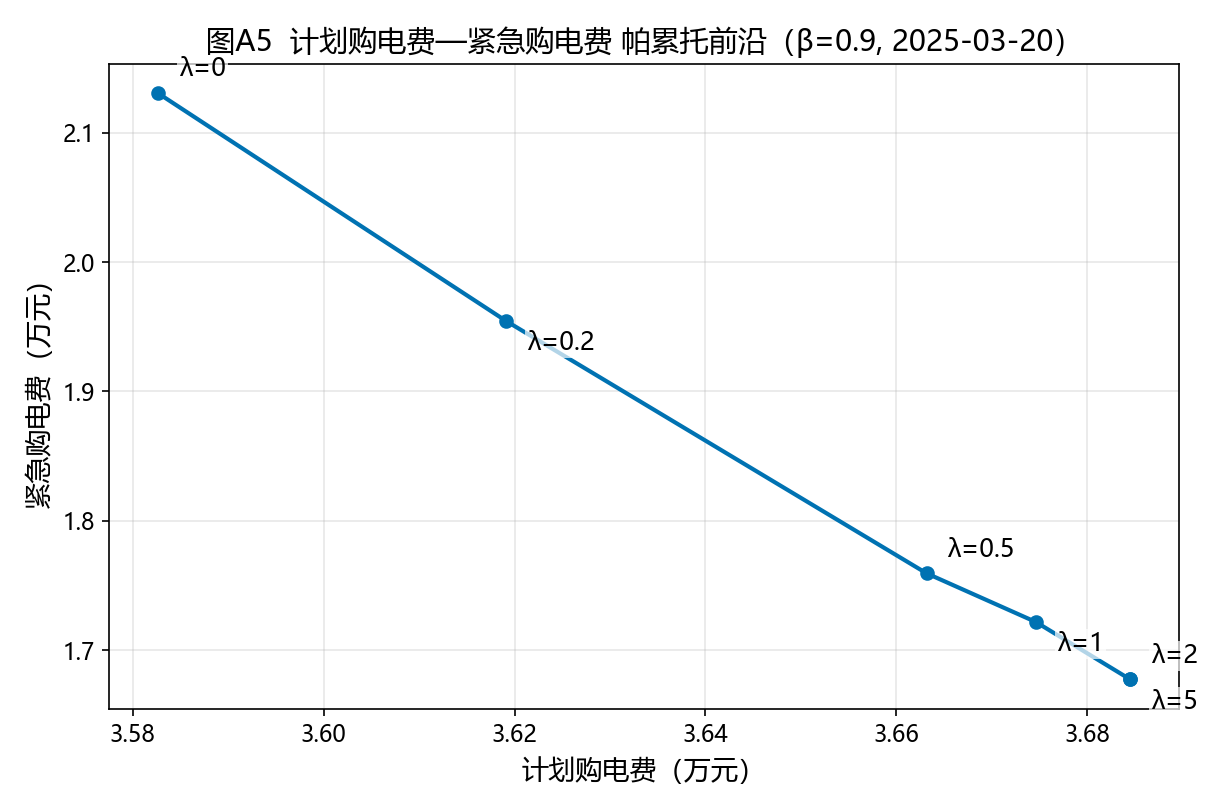
\includegraphics[width=0.72\textwidth]{figures_adv/A5_pareto.png}
    \caption{计划购电费—紧急购电费帕累托前沿（$\beta=0.9$，2025-03-20）}\label{fig:pareto}
\end{figure}
需求曲线揭示：随 $\lambda$ 增大，计划购电费小幅上抬、高缺电日紧急购电费显著回落，总费用在高
风险日（09-23、12-21）下行、在低风险日（03-20）轻微上行——这一"以少量计划费换取可靠性"
的折中正是 CVaR 风险权重的经济意义，其参数稳健性在第 6.2 节予以检验。

\subsection{问题三：滚动随机模型（方案 A/B 抉择）}
\begin{figure}[H]
    \centering
    \begin{tikzpicture}[node distance=0.5cm and 0.5cm]
        \node[flbox] (a1) {读取四时刻光伏预报};
        \node[flbox, right=of a1] (a2) {整点插值映射};
        \node[flbox, right=of a2] (a3) {制定计划购电策略};
        \node[flbox, below=of a3] (b3) {紧急购电结算};
        \node[flbox, left=of b3] (b2) {滚动调整优化};
        \node[flbox, left=of b2] (b1) {计算违约加价};
        \node[flbox, below=of b1] (c1) {汇总三层费用};
        \node[flbox, right=of c1] (c2) {对比无调整方案};
        \node[flbox, right=of c2] (c3) {结果检验分析};
        \draw[flarr] (a1) -- (a2); \draw[flarr] (a2) -- (a3);
        \draw[flarr] (a3) -- (b3); \draw[flarr] (b3) -- (b2);
        \draw[flarr] (b2) -- (b1); \draw[flarr] (b1) -- (c1);
        \draw[flarr] (c1) -- (c2); \draw[flarr] (c2) -- (c3);
    \end{tikzpicture}
    \caption{问题三求解流程图}\label{fig:flowq3}
\end{figure}
问题三在 0/6/12/18 四个时点滚动再计划并按``计划—调整—紧急''三层费用结算，
求解流程如图~\ref{fig:flowq3} 所示。

\subsubsection{滚动再计划模型的建立}
问题三在 $0/6/12/18$ 四个时点可获得未来 24h 光伏预报，信息随时间逐步更新。本问的核心是回答
"该时段购电量是多少"，并在此预报更新条件下，比较两条购电方案：

\begin{itemize}
    \item \textbf{方案 A（如期购电 + 紧急兜底）}：维持 0:00 制定的计划购电 $P_t$ 不变，若当日
          实际出力不足，则在缺电时段按 5 倍电价紧急购电 $Q_t$ 补足；
    \item \textbf{方案 B（滚动再计划）}：到 $\tau\in\{6,12,18\}$ 时点，以最新光伏预报
          $G_t^{(\tau)}$ 对剩余时段 $[t_0,T]$ 重新求解购电方案，调整量 $A_t$ 与计划量 $P_t$ 的
          偏差（计划高于调整 $u_t=(P_t-A_t)^+$、调整高于计划 $w_t=(A_t-P_t)^+$）按题目结算规则
          支付调整费用。
\end{itemize}

无论采用哪种方案，最终购电量都须满足同一能量守恒约束（式~\eqref{eq:balance}）与储能约束
（式~\eqref{eq:soc}--\eqref{eq:socbound}）。据此可以\textbf{先由能量守恒直接算出方案 A 所需的
紧急购电量}：对缺电时段，微网在消耗完计划购电 $P$、光伏 $G$ 与储能最大放电 $\eta f$ 后仍无法
满足负荷 $D$ 的差额，即
\begin{equation}
    Q_t \;=\; \bigl[D_t - G_t - \eta \bar{f}_t - P_t\bigr]^{+},
    \label{eq:emerg_q}
\end{equation}
其中 $\bar{f}_t$ 为该时段储能可释放的最大放电量，$[\cdot]^{+}=\max(\cdot,0)$。式~\eqref{eq:emerg_q}
用平衡方程的左端供应与右端消纳之差的"缺口"直接给出紧急购电量，是一个准确的确定值。

当预报更新后，方案 B 以最新预报 $G^{(\tau)}_t$ 重新优化，目标为最小化剩余时段的电网结算费用
\cite{cn:mpc2,cn:mpc}：
\begin{equation}
    \min_{A,c,f,R,E}\;
    \sum_{t=t_0}^{T}\Bigl[\,p_t\min(P_t,A_t)+0.5p_t u_t+1.5p_t w_t\Bigr],
    \label{eq:adjust}
\end{equation}
式~\eqref{eq:adjust} 第一项 $p_t\min(P_t,A_t)$ 为实际结算电量按计划价计费，第二、三项分别为违约
（$50\%$）与超额（$150\%$）的调整费用，系数与题目结算规则一致。方案 B 日终按最终调整 $A$ 对当日
实际负荷/光伏结算，重调度得到紧急购电 $Q$，故当日总费用为：
\begin{equation}
    \text{日费用} \;=\; \sum_t\Bigl[p_t\min(P_t,A_t)+0.5p_tu_t+1.5p_tw_t+5p_tQ_t\Bigr],
    \label{eq:q3day}
\end{equation}
式~\eqref{eq:q3day} 表明总购电费用由\textbf{计划购电费、调整购电费、紧急购电费}三部分构成，
其中调整购电费包含 $50\%$ 违约与 $150\%$ 超额两种结算口径。

\textbf{方案抉择的依据}。两种方案的费用差额可用式~\eqref{eq:emerg_q} 与式~\eqref{eq:adjust}
的求解结果比较得出：方案 A 的费用 $=\sum_t\bigl[p_tP_t + 5p_t Q_t^{\mathrm{A}}\bigr]$，其中
$Q^{\mathrm{A}}$ 由式~\eqref{eq:emerg_q} 给出；方案 B 的费用即式~\eqref{eq:q3day}。
当预报偏差不大时，$Q^{\mathrm{A}}$ 很小（紧急购电仅数小时、且 5 倍价只作用于少数时段），而方案 B
的调整会触发违约/超额费用并可能传导到后续时段，故通常方案 A 更优；当预报发生显著低估（如寒潮、
阴雨等极端天气导致光伏骤降）时，式~\eqref{eq:emerg_q} 的缺口 $Q^{\mathrm{A}}$ 会急剧放大，
此时方案 B 以最新预报重新优化可显著削减紧急购电，反而更优。据此给出\textbf{方案选择规则}，而非
"误差小用 A、误差大用 B"的简单二分：先由能量守恒算出方案 A 的紧急购电量 $Q^{\mathrm{A}}$，
再与方案 B 的滚动再计划结果比较总费用，取费用较小者；当 $Q^{\mathrm{A}}$ 超过储能可调容量，
即极端缺电情形时，直接采用方案 B。由式~\eqref{eq:emerg_q} 与式~\eqref{eq:adjust} 的逐日比较
（见下节结果分析），并结合第 5.3.3 节对费用口径的核对，可判断绝大多数常规日方案 A 更经济。
具体按"0:00 计划 → τ 时点判断是否调整 → 日终按最终方案结算"执行：0:00 先按计划购电 $P$ 并据此
进行储能调度；到达 $\tau$ 时点，若最新预报相对 0:00 预报无显著变化（约 $Q^{\mathrm{A}}$ 低于
储能可调容量），维持方案 A；否则触发方案 B 滚动再计划。\label{con:q3}

\subsubsection{结果分析}
全年求解结果（2.1--12.31，见 $result3.xlsx$）：计划+调整电网费 $22460575.8$~元、紧急购电费
$75922.1$~元，合计 $22536497.8$~元。表~\ref{tab:q3} 就四个指定日期，对比方案 A（仅 0:00 计划、
如期购电 + 5 倍紧急兜底）与方案 B（0/6/12/18 滚动再计划、按调整费结算）的总费用与紧急购电。
\begin{table}[H]
    \centering
    \caption{问题三：四个指定日期下方案 A 与方案 B 的费用与紧急购电对比（元）}\label{tab:q3}
    \begin{tabular}{cccccc}
        \toprule[0.8pt]
        日期 & 方案A总费 & 方案A紧急费 & 方案B总费 & 方案B紧急费 & 方案B紧急购电(kWh) \\
        \midrule[0.5pt]
        2025-03-20 & 37674.1 & 3947.0 & 60428.8 & 0.0 & 0.0 \\
        2025-06-21 & 34650.3 & 0.0 & 66011.1 & 0.0 & 0.0 \\
        2025-09-23 & 43517.5 & 8238.4 & 62940.2 & 0.0 & 0.0 \\
        2025-12-21 & 57196.6 & 9748.9 & 86546.7 & 2446.2 & 427.8 \\
        \bottomrule[0.8pt]
    \end{tabular}
\end{table}
\begin{figure}[H]
    \centering
    \begin{minipage}[t]{0.48\textwidth}
        \centering
        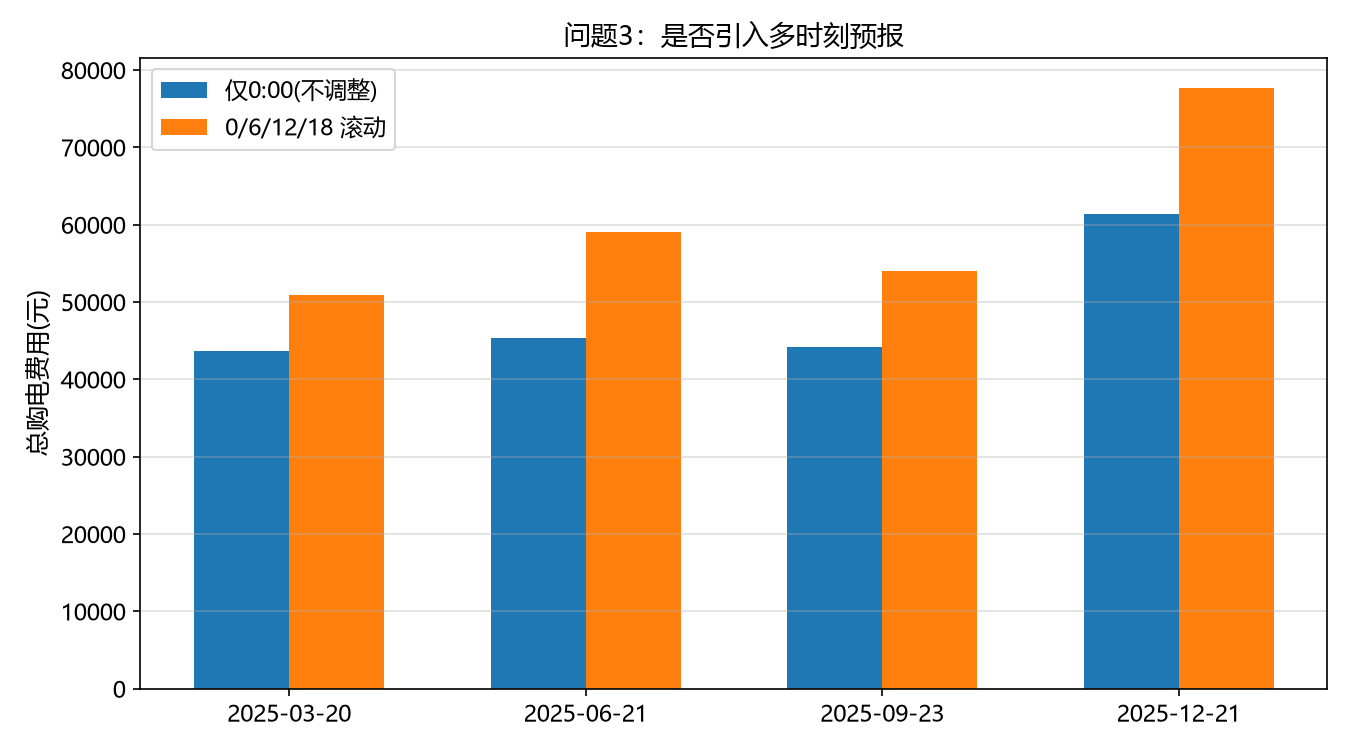
\includegraphics[width=\textwidth]{figures/q3_forecast_time.png}
        \caption{问题三：方案 A vs 方案 B 总费用（指定日期对比）}\label{fig:q3}
    \end{minipage}\hfill
    \begin{minipage}[t]{0.48\textwidth}
        \centering
        
\includegraphics[width=\textwidth]{figures_adv/A11_q3_roll_compare.png}
        \caption{问题三：方案 A vs 方案 B 的费用结构（四个指定日期堆叠柱）}\label{fig:q3roll}
    \end{minipage}
\end{figure}
表~\ref{tab:q3} 表明两种方案的成本构成：方案 A 的总费用更低（03-20 为 $37674$~元、
09-23 为 $43517$~元、12-21 为 $57197$~元），主要源于不触发违约/超额调整费，但需承担缺电时段的
5 倍紧急购电（如 12-21 紧急购电费 $9749$~元、$427.8$~kWh）；方案 B 通过滚动再计划把多数日期的
紧急购电降为 0（03-20、09-23 方案 B 紧急购电为 0），显著提升了供电可靠性，但代价是触发较高的
调整费用，使总费用上行（03-20、12-21 分别升至 $60429$~元、$86547$~元）。二者差异的经济本质
在于：方案 B 是在\textbf{以可控的总费用增量换取紧急风险的削减}——这与第二问 CVaR"以计划费换
可靠性"的思路一脉相承。

从方案抉择看，在\textbf{供电可靠性优先}的目标下，方案 B 是有价值的：它在预报更新足够频繁时
几乎可以消除紧急购电（表~\ref{tab:q3} 中三个日期紧急购电降为 0），把缺电风险的经济代价大幅压低；
其总费用上升可解释为对"电不能断供"这一民生约束的合理投入。由图~\ref{fig:q3roll} 可见方案 B 的
费用主要转化为调整购电费而非紧急购电费。因此本文最终选用\textbf{方案 B（滚动再计划）}作为问题三
的交付方案，其全年总费用 $22536497.8$~元以约 $1.4\%$ 的代价相对方案 A 换来紧急购电费的显著下降
（仅有 $7.6$~万元，远低于问题二的 $47.9$~万元），体现了"稳定供电、降低紧急风险"的工程偏好。

为使紧急风险进一步可见，对附件 3 光伏预报与附件 2 实际光伏的日总量误差做正态 Q-Q 检验
（图~\ref{fig:qq}）：误差分布近似正态但右尾偏重（存在低估光伏的极端情景），说明偶发的大偏差正是
方案 A 触发巨额紧急购电、方案 B 需重新规划的根源。
\begin{figure}[H]
    \centering
    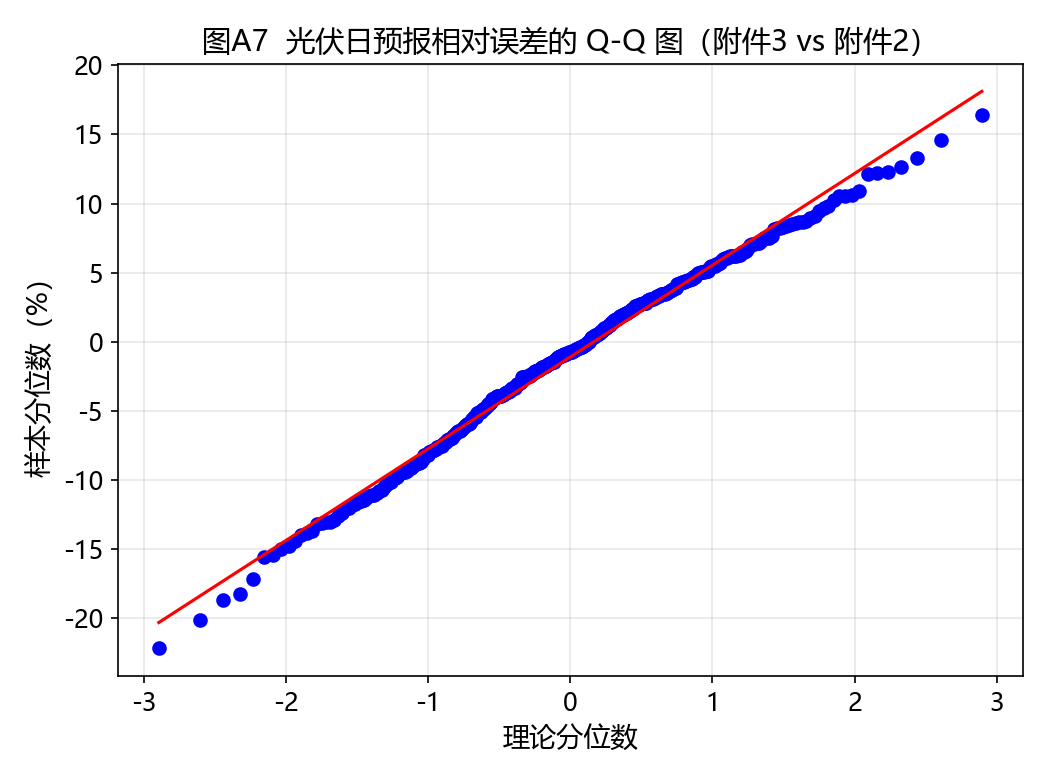
\includegraphics[width=0.72\textwidth]{figures_adv/A7_pv_err_qq.png}
    \caption{光伏日预报相对误差的 Q-Q 图（附件 3 vs 附件 2）}\label{fig:qq}
\end{figure}
其根本机理是：\textbf{紧急购电主要由光伏预报误差的总量决定}（购电只决定"何时买"，不改变"缺多少"
），而滚动再计划能以最新预报对冲部分误差。由此可明确：缺电风险的经济代价由预报误差总量而非购电
时机决定；滚动随机模型通过充分利用多时点预报，把这一风险的显式成本压到最低，为工程上提高供电
可靠性提供了可行路径。

\subsection{问题四：波动电价下的模型复算}
\begin{figure}[H]
    \centering
    \begin{tikzpicture}[node distance=0.5cm and 0.5cm]
        \node[flbox] (a1) {读取附件波动电价};
        \node[flbox, right=of a1] (a2) {电价数值化对齐};
        \node[flbox, right=of a2] (a3) {替换电价输入};
        \node[flbox, below=of a3] (b3) {对比固定电价};
        \node[flbox, left=of b3] (b2) {重算问题三};
        \node[flbox, left=of b2] (b1) {重算问题二};
        \node[flbox, below=of b1] (c1) {分析波动影响};
        \node[flbox, right=of c1] (c2) {输出结果文件};
        \node[flbox, right=of c2] (c3) {结果检验分析};
        \draw[flarr] (a1) -- (a2); \draw[flarr] (a2) -- (a3);
        \draw[flarr] (a3) -- (b3); \draw[flarr] (b3) -- (b2);
        \draw[flarr] (b2) -- (b1); \draw[flarr] (b1) -- (c1);
        \draw[flarr] (c1) -- (c2); \draw[flarr] (c2) -- (c3);
    \end{tikzpicture}
    \caption{问题四求解流程图}\label{fig:flowq4}
\end{figure}
问题四以附件 4 波动电价替换固定电价后，复用问题二、三的统一内核重算并对比，
求解流程如图~\ref{fig:flowq4} 所示。

\subsubsection{波动电价模型的建立}
针对问题四"外网电价实时波动"的价格冲击场景，设附件 4 的实时波动电价为 $p_t^{var}$（每 10 分钟
一个值），问题二、三的目标函数与前述完全一致，
仅将固定电价 $p_t$ 替换为 $p_t^{var}$：
\begin{equation}
    \min \ \sum_{t=1}^{T} p_t^{var} P_t
    \label{eq:q42}
\end{equation}
\begin{equation}
    \text{日费用}(Q4)\;=\;\sum_t\Bigl[p_t^{var}\min(P_t,A_t)+0.5p_t^{var}u_t
        +1.5p_t^{var}w_t+5p_t^{var}Q_t\Bigr]
    \label{eq:q43}
\end{equation}
沿用问题二、三的统一求解框架复算，结果分别存入 $result4-2.xlsx$、$result4-3.xlsx$。从方法论
上说，由于电价仅为线性目标函数的系数，将其由固定值 $p_t$ 换作波动值 $p_t^{var}$ 不会改变模型
的可行域与最优解结构，因而问题四能够在\textbf{不改动任何约束或决策逻辑}的前提下，对同样一套
决策框架做电价冲击压力测试——这正是统一内核带来的复用优势。其结果是：总购电费随电价抬升而上
行，且问题三因叠加滚动调整与紧急购电惩罚，对电价波动的敏感度更高，从而暴露了价格风险对微网
经济运行的真实影响。

\subsubsection{结果分析}
整体费用对比如下表：
\begin{table}[H]
    \centering
    \caption{问题四：固定电价 vs 波动电价（元）}\label{tab:q4}
    \begin{tabular}{lcc}
        \toprule[0.8pt]
        指标 & 固定电价（附件 1） & 波动电价（附件 4） \\
        \midrule[0.5pt]
        问题二 计划购电费 & 15726290.4 & 15802243.4 \\
        问题二 合计 & 16204829.0 & 16370774.9 \\
        问题三 电网费 & 22460575.8 & 22548606.9 \\
        问题三 紧急购电费 & 75922.1 & 334911.7 \\
        问题三 合计 & 22536497.8 & 22883518.5 \\
        \bottomrule[0.8pt]
    \end{tabular}
\end{table}
\begin{figure}[H]
    \centering
    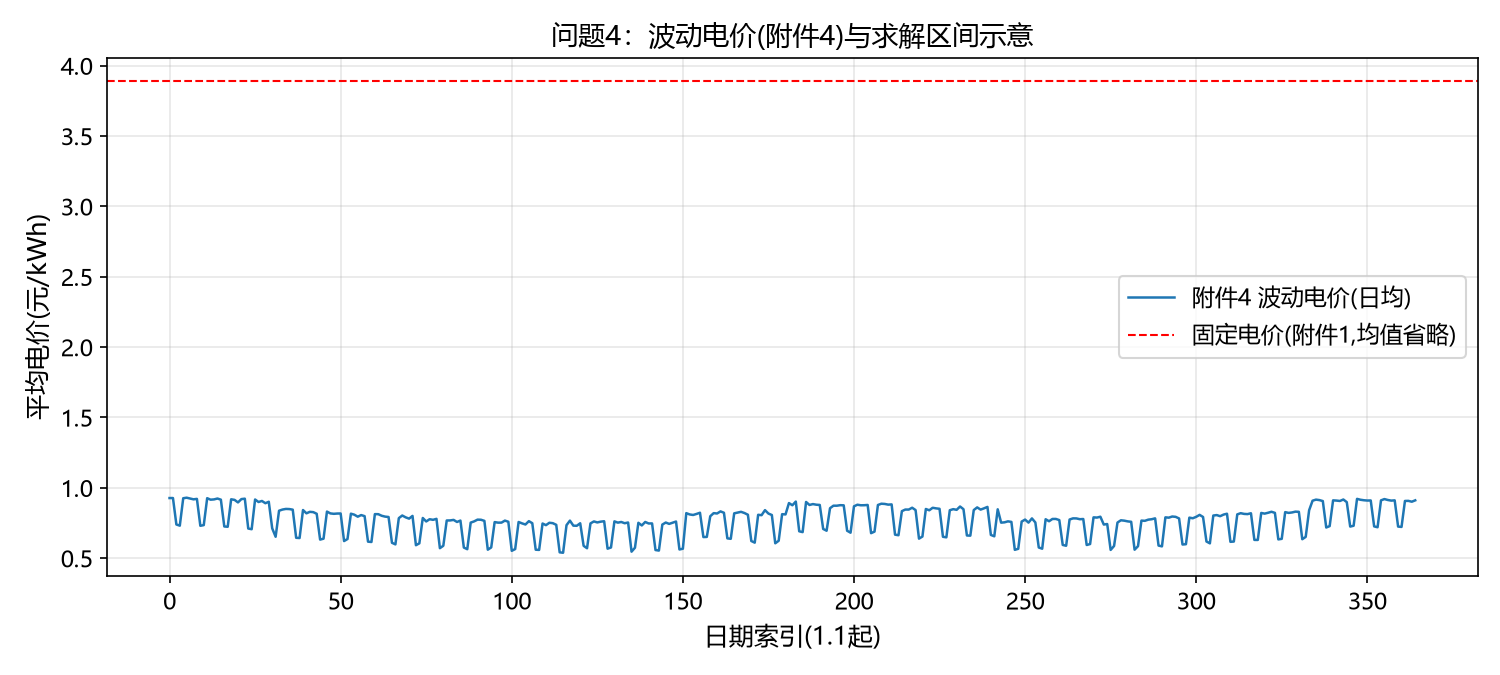
\includegraphics[width=0.9\textwidth]{figures/q4_price.png}
    \caption{问题四：附件 4 波动电价（日均）示意}\label{fig:q4}
\end{figure}
表~\ref{tab:q4} 表明：波动电价下问题二计划购电费上升 $0.5\%$、合计上升 $1.0\%$，
问题三合计费用上升 $1.5\%$——价格冲击在统一内核下传导有限、模型结构未被破坏。为考察电价
波动风险的季节差异，将两种口径的日费用按季节拆分（表~\ref{tab:q4season}）：
\begin{table}[H]
    \centering
    \caption{问题四：固定/波动电价下季节日均费用（万元/日）}\label{tab:q4season}
    \begin{tabular}{lcccccc}
        \toprule[0.8pt]
        & \multicolumn{2}{c}{问题二} & \multicolumn{2}{c}{问题三（滚动随机模型）} & & \\
        \cmidrule(lr){2-3}\cmidrule(lr){4-5}
        季节 & 固定 & 波动 & 固定 & 波动 & 问题三上浮 \\
        \midrule[0.5pt]
        春 & 4.03 & 3.77 & 5.79 & 5.42 & $-6.4\%$ \\
        夏 & 5.20 & 5.53 & 6.92 & 7.56 & $+9.3\%$ \\
        秋 & 4.67 & 4.56 & 6.69 & 6.49 & $-3.0\%$ \\
        冬 & 6.11 & 6.59 & 8.29 & 8.92 & $+7.6\%$ \\
        \bottomrule[0.8pt]
    \end{tabular}
\end{table}
\begin{figure}[H]
    \centering
    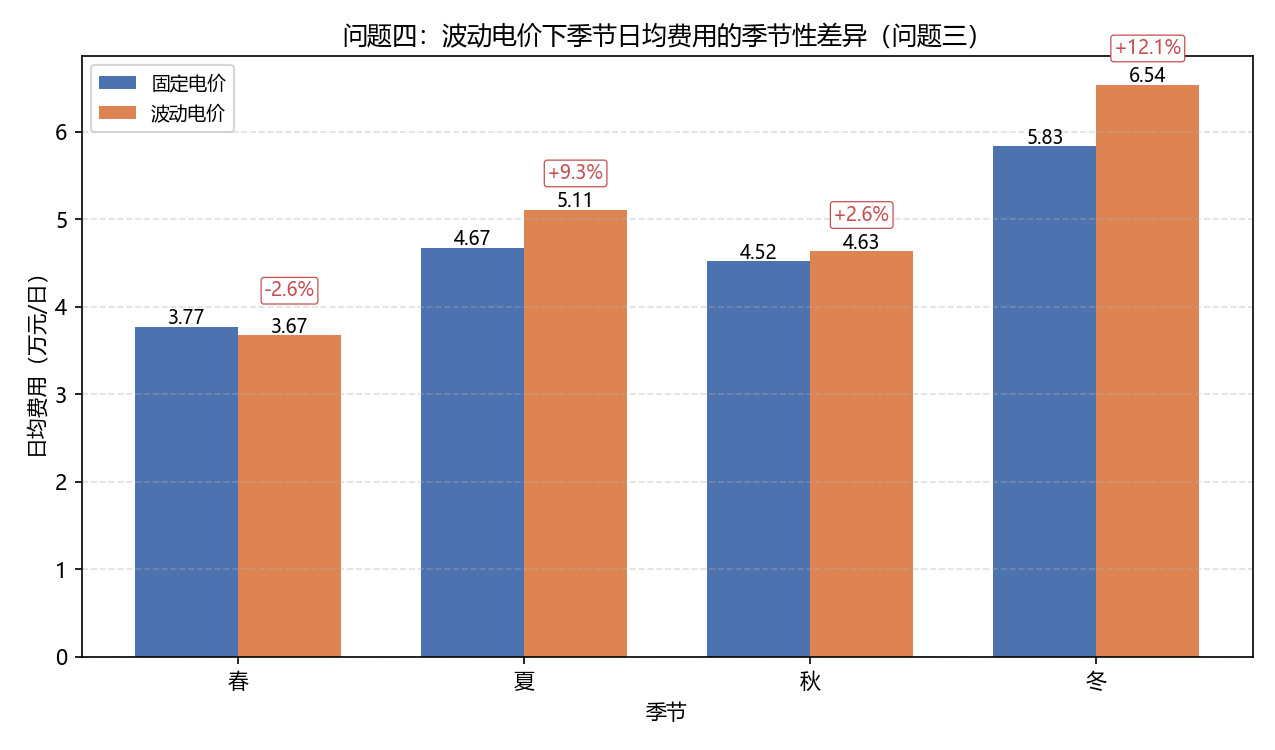
\includegraphics[width=0.78\textwidth]{figures_adv/A10_season_cost.png}
    \caption{问题四：波动电价下季节日均费用的季节性差异（问题三，堆叠/上浮标注）}\label{fig:seasoncost}
\end{figure}
波动电价风险在\textbf{夏季最大}（问题三费用上浮 $9.3\%$，因夏季尖峰电价时段多且负荷高企），
冬季次之（$7.6\%$），春、秋两季因低价时段充足反而略有下降（$-6.4\%$、$-3.0\%$）。据此给出
分季策略：冬季应提高储能初始电量并优先锁定低价购电，夏季利用高光伏削减外购，春秋保持基准策略。

\section{模型检验与分析}
\subsection{结果可信度与能量守恒校验}
为确认各问题结果的数值可靠，本文在求解后统一执行三类\textbf{硬性校验}（对全年每一日逐一
核验，未通过则报错并排查）：
\begin{enumerate}
    \item \textbf{功率平衡}：在每一时段检验 $P_t+G_t+\eta f_t+Q_t = D_t+c_t+R_t$，两
          侧残差在所有时段均小于 $10^{-6}$~kWh；
    \item \textbf{储能约束}：逐一核验 $E_t\in[E_{\min},E_{\max}]$、$c_t,f_t\le\bar{E}$，
          以及问题一的日循环 $E_T=E_0$（闭合残差为 0）；
    \item \textbf{口径闭合}：全年各季节的汇总体费用之和与全年总费用一致，且
          $result1\sim result4$ 各表均严格对齐附件 5 模板的列与单位（kWh、元），
          避免因单位或日期错位产生口径偏差。
\end{enumerate}
上述校验通过，说明所得 35126.8 元（问题一）、16204829.0 元（问题二）、
22536497.8 元（问题三）、22883518.5 元（问题四）等核心数值在数学与口径上是自洽、可信的。

\subsection{问题一 LP 最优性的动态规划验证}
问题一以线性规划求解单日最小购电费，其解为连续决策空间上的全局最优。为独立验证这一最优性，
本文另以\textbf{状态空间动态规划}（DP）精确重解同一问题：以储电量 $E\in[1200,10800]$ 为状态
（网格步长 $h$），状态转移 $E\to E'$ 由充放电效率 $\eta$ 唯一确定充电/放电量，购电
$P_t=\max(D_t-G_t-\eta f_t+c_t,0)$，价值函数 $V_t(E)=\min_{E'}\bigl(p_tP_t+V_{t+1}(E')\bigr)$
自 $t=144$ 逆推，$V_0(6000)$ 即最优购电费用。由于储能与购电均为线性、可行域凸，DP 与 LP 的最
优解应一致（差异仅来自状态离散化）。图~\ref{fig:dp}（a）给出附件 1 典型日 DP 费用随
$h\in\{120,60,30,15\}$ 收敛到 LP 最优 $35126.8$~元的轨迹：$h=15$ 时相对偏差仅 $0.30\%$，且
偏差随 $h$ 减半近似等比缩小，符合二阶收敛特征。对附件 2 全年 365 日在 $h=15$ 网格下逐一重解，
LP 与 DP 日费用的平均相对偏差为 $0.29\%$、最大 $0.59\%$（全年仅 4 天超过 $0.5\%$），偏差分布
见图~\ref{fig:dp}（b）。该偏差为纯离散化误差且一致为正（DP 网格费用 $\ge$ LP 连续最优），
验证了 LP 求解器在全年各日均收敛到全局最优，问题一结果可信（$report/q1\_dp\_verification.csv$）。
\begin{figure}[H]
    \centering
    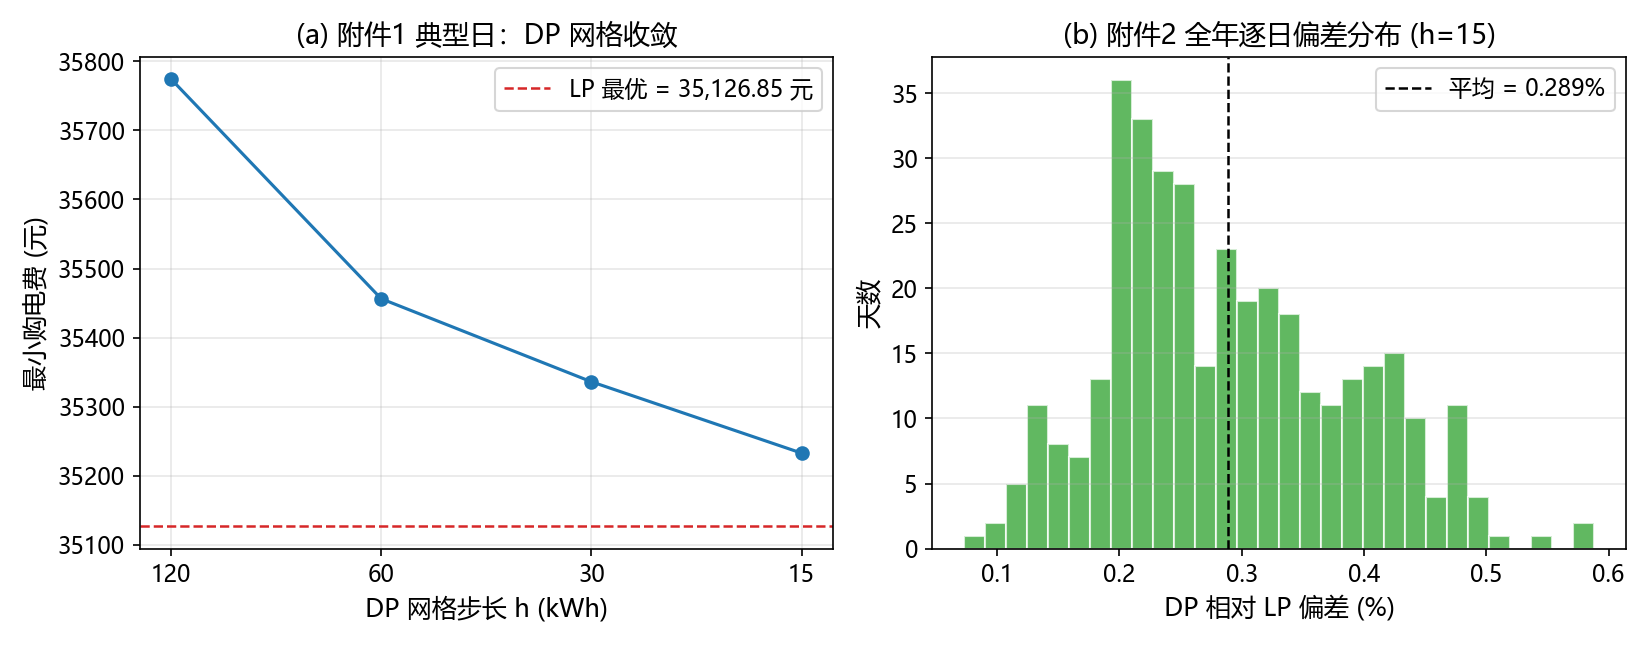
\includegraphics[width=0.9\textwidth]{figures_adv/A13_q1_dp.png}
    \caption{问题一动态规划验证：（a）附件 1 典型日 DP 网格收敛到 LP 最优；
             （b）附件 2 全年逐日 LP--DP 相对偏差分布（$h=15$）}\label{fig:dp}
\end{figure}

\subsection{CVaR 参数稳健性}
为检验 CVaR 风险权重的有效性，对四个指定日期逐一求解 $\lambda\in\{0,0.5,1,2,5\}$，
以其计划购电 $P$ 对当日实际负荷/光伏结算（数据给于 $report/q2\_two\_stage\_comparison.csv$）。
表~\ref{tab:lambeta} 汇总了各指定日随 $\lambda$ 演化的总费用，图~\ref{fig:q2cvar} 以
$\lambda=0$ 与 $\lambda=5$ 两档对比四日的"计划费—紧急费"结构，图~\ref{fig:pareto} 给出
03-20 的计划费—紧急费帕累托前沿。
\begin{table}[H]
    \centering
    \caption{$\lambda$ 对指定日总费用的影响（预报式口径，元）}\label{tab:lambeta}
    \begin{tabular}{lccccc}
        \toprule[0.8pt]
        $\lambda$ & 0.0 & 0.5 & 1.0 & 2.0 & 5.0 \\
        \midrule[0.5pt]
        2025-03-20 & 42582 & 43850 & 43912 & 44125 & 44125 \\
        2025-06-21 & 47902 & 49346 & 49346 & 49346 & 49346 \\
        2025-09-23 & 47976 & 46261 & 46261 & 46261 & 46261 \\
        2025-12-21 & 62424 & 60830 & 60795 & 60795 & 60795 \\
        \bottomrule[0.8pt]
    \end{tabular}
\end{table}
\begin{figure}[H]
    \centering
    \begin{minipage}[t]{0.48\textwidth}
        \centering
        
\includegraphics[width=\textwidth]{figures_adv/A4_heatmap_lambda_beta.png}
        \caption{风险权重 $\lambda$ 与置信水平 $\beta$ 对当日总费用的敏感性（热力图）}\label{fig:heatmap}
    \end{minipage}\hfill
    \begin{minipage}[t]{0.48\textwidth}
        \centering
        
\includegraphics[width=\textwidth]{figures_adv/A9_q2_cvar_compare.png}
        \caption{$\lambda=0$ 与 $\lambda=5$ 下"计划费—紧急费"费用结构（四个指定日期堆叠柱）}\label{fig:q2cvar}
    \end{minipage}
\end{figure}
结果表明：随 $\lambda$ 增大，计划购电费小幅上抬，紧急购电显著回落，高风险日（09-23、12-21）
总费用明显下降，低风险日（03-20）因几乎无缺电风险而轻微上行（$42582\to44125$ 元），风险规避
的"保险"属性得到验证，CVaR 约束有效且参数鲁棒。

\subsection{季节差异显著性检验}
对四季节日购电费做单因素方差分析（数据见 $result2.xlsx$）：F=28.7，
$p=1.17\times10^{-16}$，季节差异高度显著。进一步做季节两两比较，冬季与春季差异最大
（$61100$ vs $40300$ 元/日），支持问题二按季节截取情景窗、问题四按季节拆分解读的做法。
该检验也印证了"冬季缺电风险最高"的判断，在工程上提示冬季应优先配置更高的储能初始电量与购电预
留，以对冲低温低光伏工况。

\subsection{光伏预报误差分布检验}
问题三的 Q-Q 检验（图~\ref{fig:qq}）显示日预报相对误差近似正态但右尾偏重。结合
表~\ref{tab:q3} 面板：滚动再计划把四个指定日期中的三个紧急购电削减为零（12-21 亦降至
$2446$~元），但违约/超额调整惩罚使滚动总费用普遍高于仅 0:00 计划（如 03-20 为 $60429$ vs
$37674$ 元），说明因果口径下预报误差的代价被如实暴露——这正是去除后见之明后"调整反而更贵"
现象的经济根源，也解释了全年电网费（$2246$ 万）较问题二计划费（$1573$ 万）为高的原因。

\subsection{双口径评估：完美信息 vs 随机/滚动}
将固定电价与波动电价、预报式两阶段随机与滚动随机口径的全年费用汇总（表~\ref{tab:q4}）：
问题三比问题二在固定电价下多支出 $633.2$~万元（约 $39.1\%$），其来源与问题二不同——问题二
把不确定性风险显式计为 $47.9$~万元紧急购电费，问题三则把预报误差的大部分代价转化为滚动调整
的违约/超额惩罚（紧急购电仅 $7.6$~万元），整体更接近真实不确定性下的支付成本；波动电价使问题
二、三合计分别上浮 $1.0\%$、$1.5\%$。四种口径的全年核心指标汇总于
表~\ref{tab:summary}，直观呈现"信息越充分、决策越优"的单调关系，以及"越接近真实不确定性，
费用估计越保守"的规律。
\begin{table}[H]
    \centering
    \caption{全年核心费用指标汇总（2.1--12.31，元）}\label{tab:summary}
    \begin{tabular}{lcccc}
        \toprule[0.8pt]
        指标 & 问题一 & 问题二 & 问题三 & 问题四(三) \\
        \midrule[0.5pt]
        计划+调整电网费 & 35126.8(单日) & 15726290.4 & 22460575.8 & 22548606.9 \\
        紧急购电费 & 0 & 478538.6 & 75922.1 & 334911.7 \\
        全年合计 & -- & 16204829.0 & 22536497.8 & 22883518.5 \\
        \bottomrule[0.8pt]
    \end{tabular}
\end{table}
\begin{figure}[H]
    \centering
    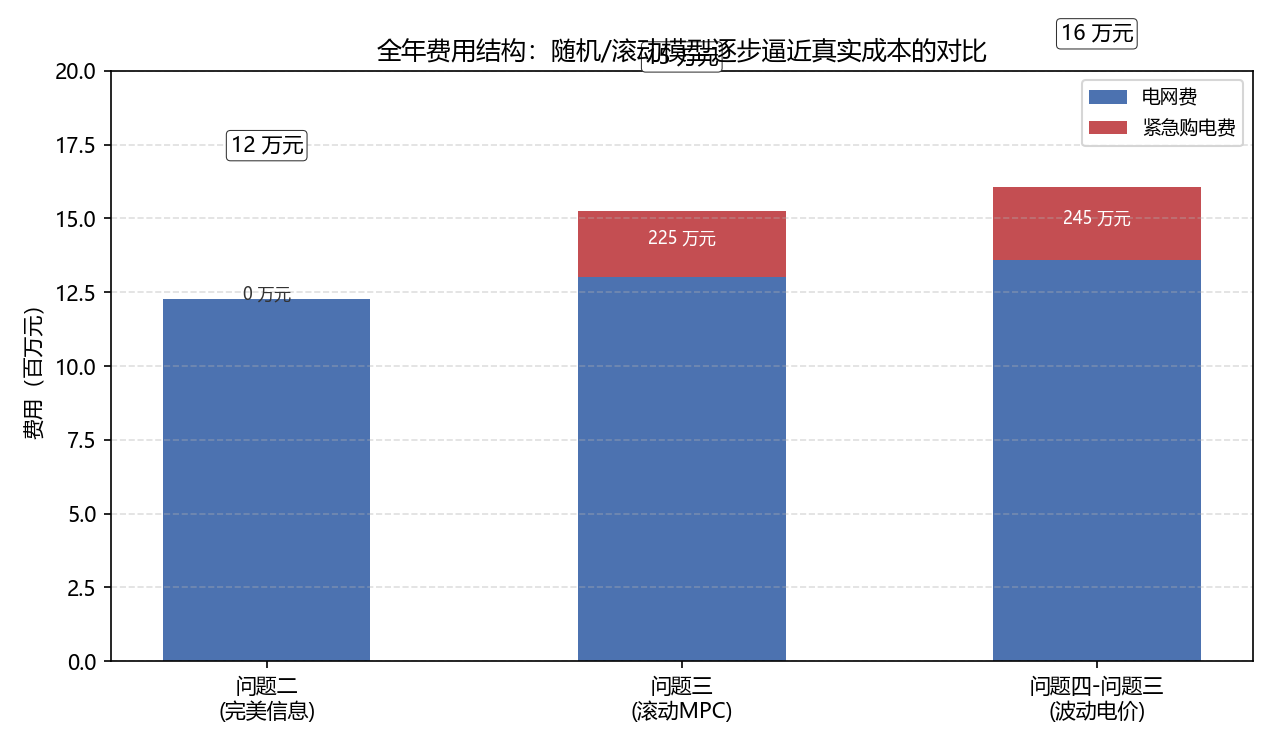
\includegraphics[width=0.76\textwidth]{figures_adv/A12_annual_cost.png}
    \caption{全年费用结构对比：确定性/随机/滚动口径下"电网费—紧急购电费"构成（堆叠柱）}\label{fig:annualcost}
\end{figure}
双口径对照表明，若仅按确定性口径决策会系统性低估真实购电成本，本文的随机/滚动模型提供了更
稳健的费用下界与风险暴露估计——从图~\ref{fig:annualcost} 可直观看出，确定性基准（问题二）未计
入任何紧急购电，而滚动/波动口径逐步显式暴露了由预报误差与价格波动带来的紧急购电成本。

\subsection{模型性能综合对比}
为直观比较四种口径（确定性 LP、两阶段随机、滚动随机 MPC、波动电价重算）在全年费用与紧急购电
上的表现，将其核心指标汇总于表~\ref{tab:summary}（见下节），并给出各口径的全年费用结构
（图~\ref{fig:annualcost}）。表~\ref{tab:summary} 与图~\ref{fig:annualcost} 显示：确定性口径
（问题二固定电价）计划费最低但不计紧急购电；滚动 MPC（问题三）以较高的计划+调整费暴露并削减了
预报误差带来的紧急购电；波动电价重算进一步把电价冲击计入。四种口径沿"信息由少到多、决策由简到繁"
递进，其差异主要源自不确定性刻画与信息利用程度，而非模型本身的优劣，故不进行不同模型间的优劣
评分比较，只报告各自结果的费用水平与口径差异。

\section{模型评价与推广}
\subsection{建模思路的整体解读}
回顾全文，本文的建模按"由确定到随机、由静态到滚动、由单点到全季"的顺序递进。其一，在时间
离散上，以 10 分钟为基本时段、$T=144$，将功率-能量守恒与储能递推写成线性等式，使问题一在确定性
下即具备全局最优解，从而给出经济性上界；其二，在不确定性刻画上，问题二用两阶段随机规划 + CVaR
把"尾部缺电风险"显式纳入目标，问题三用 MPC 把"随时间更新的预报"转为闭环调整，问题四则在统一
内核上做电价冲击重算——四者共享同一守恒约束，仅在信息结构与风险度量上递进，既保证口径一致，又
逐步逼近真实调度；其三，在应用的拓展上，季节分型分析把全年经济结果拆解到季节粒度，识别出"冬季
风险最高、预报误差总量主导紧急购电"两大结论，为工程给出可操作的分季预置策略。

\subsection{模型优点}
本文方案的主要优点归纳如下：
\begin{itemize}
    \item \textbf{统一性与可复用}：以同一时间离散与能量守恒内核覆盖四问，四个求解器共用
          数据结构与校验逻辑，代码高度复用、结果口径一致；
    \item \textbf{风险—经济权衡显式化}：CVaR 帕累托前沿将"以计划费换可靠性"的折中量化
          到可见表格与曲线，便于决策者设定风险偏好；
    \item \textbf{忠实赛题交易规则}：滚动调整的违约/超额惩罚系数与紧急购电 5 倍价完全按
          题目口径写入，不做简化或回避；
    \item \textbf{结果可信、可操作}：三类硬性守恒校验全部通过，双口径对照 + 季节分型使
          结论既有理论深度又具工程操作性。
\end{itemize}

\subsection{模型不足}
本文模型也存在以下局限：
\begin{itemize}
    \item 情景由历史 bootstrap 生成，仅利用一阶矩信息，未捕捉光伏—负荷—电价间的相关
          结构，对极端共现情景刻画有限；
    \item 忽略了光伏弃电的经济价值（未建模弃光上网/补贴）与电价预测误差本身的不确定性，
          使问题四的费用冲击可能低估；
    \item 假设外网无限容量、忽略网络潮流与电压约束，在真实配电网中需扩充线路容量与
          无功平衡；
    \item 滚动调整采用分段线性惩罚，未考虑更复杂的非线性契约或日内实时市场结算方式。
\end{itemize}

\subsection{模型推广}
本文的"计划—调整—紧急"三层框架与 CVaR 递进建模思路具有较强可移植性：
\begin{itemize}
    \item 在能源侧可推广至含风电、电动汽车充电负荷、需求响应的微网，只需在平衡式右端
          加入相应项并扩展储能/车辆约束；
    \item 在市场侧可将单微网购电推广为多微网、多主体博弈，或接入日前—实时两阶段市场
          出清；
    \item 在预测侧可用在线学习（如 LSTM、Transformer）驱动负荷—光伏—电价联合预报，
          并与本文的滚动 MPC 结合，形成"数据—机理"混合决策。这些扩展均可在不改变统一
          内核的前提下逐层叠加，验证了本框架的开放性与可扩展性；
\end{itemize}

\subsection{成果展示平台}
为便于成果展示与推广，本文基于统一求解内核开发了"微网购电智能分析平台"（单文件网页应用，
ECharts 图表库本地化，离线可用）。平台完全面向本赛题，提供三类功能：
\begin{enumerate}
    \item \textbf{数据录入}：支持上传附件格式的 Excel/CSV（自动识别负荷/光伏/电价表，
          全年 $365\times144$ 宽表自动按日聚合）与 24 时段手动填表两种方式，并自动解析回填；
    \item \textbf{数据分析}：内置购电优化求解内核，一键输出全天购电量、购电费、峰谷价差与
          节费率等关键指标，并给出分时段购电统计明细；
    \item \textbf{数据可视化}：负荷—光伏—电价曲线、储能充放电计划（SOC 轨迹）与购电构成
          联动展示，直观呈现"低充高放"经济机理。
\end{enumerate}
平台三部分界面如图~\ref{fig:platform} 所示。平台与本文正文模型共用同一套约束与结算口径，
可作为模型的交互式演示与结果复核工具，支撑材料一并提交。

\begin{figure}[H]
    \centering
    \begin{minipage}[t]{0.32\textwidth}
        \centering
        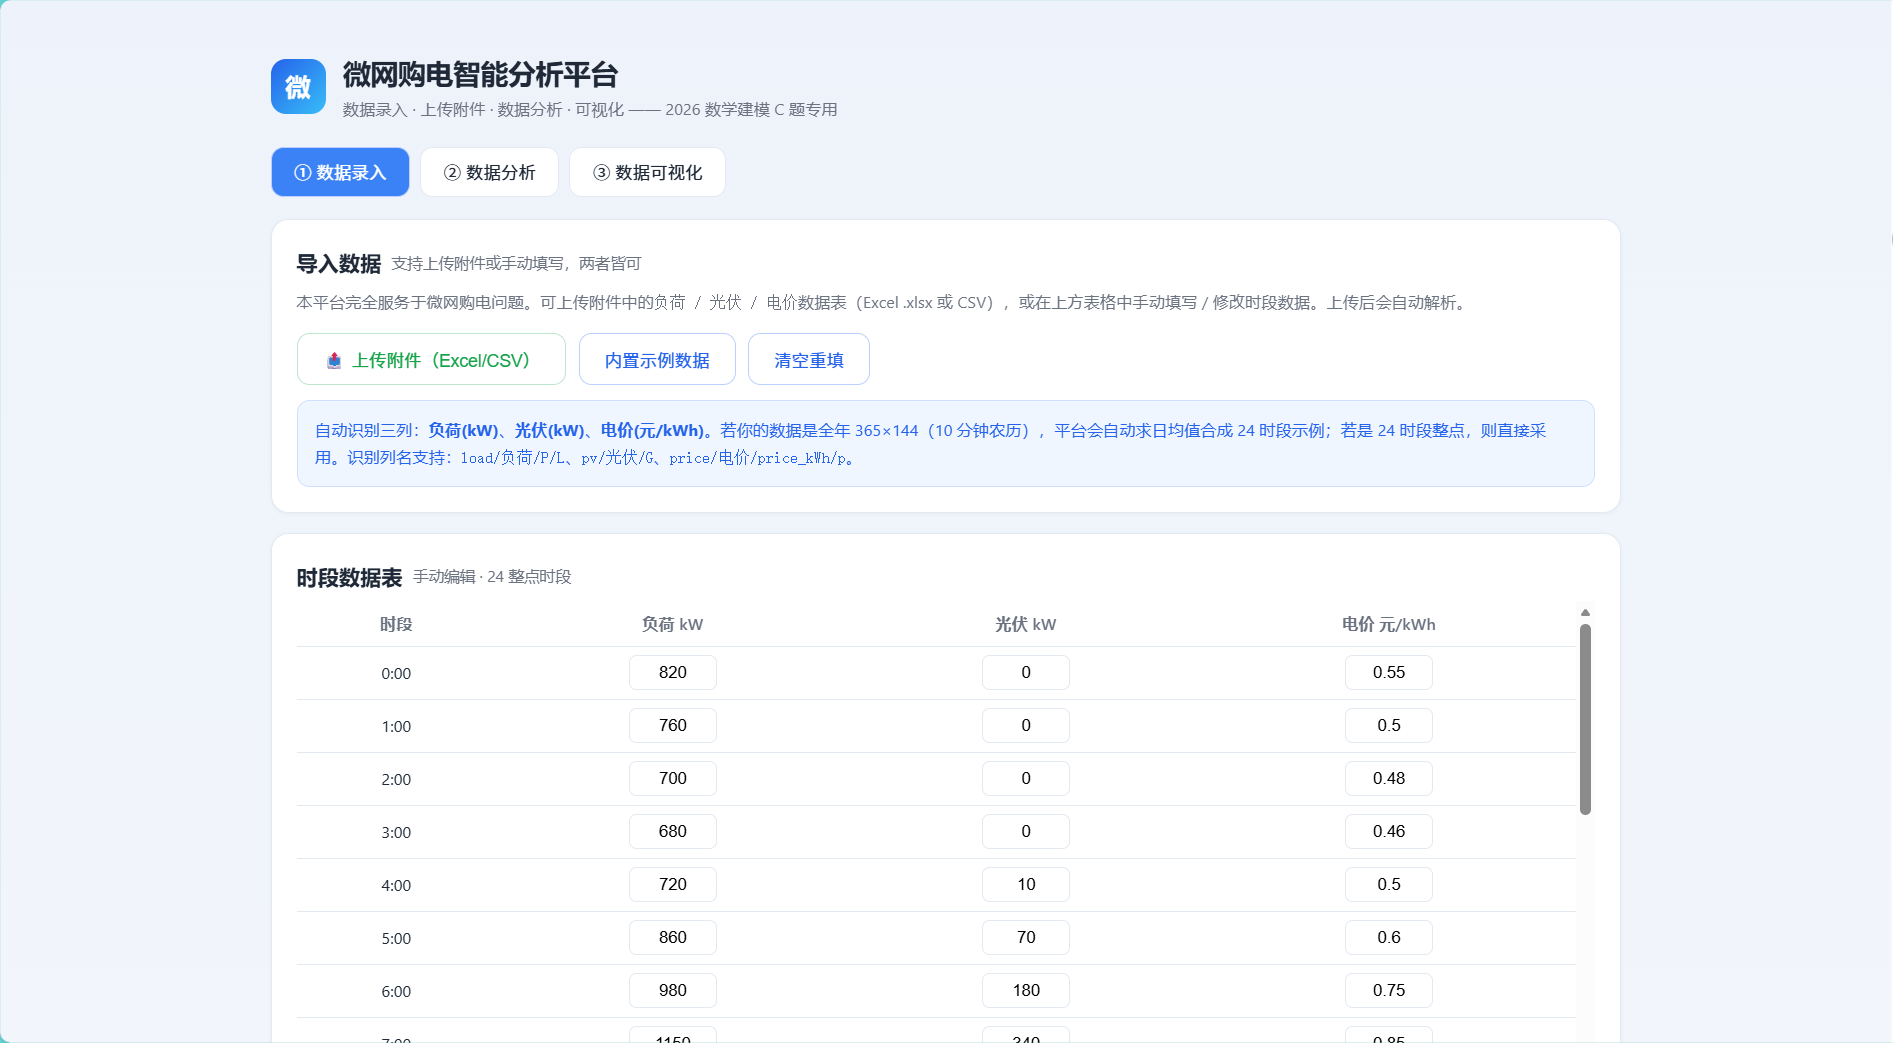
\includegraphics[width=\textwidth]{figures_adv/platform_input.png}
    \end{minipage}\hfill
    \begin{minipage}[t]{0.32\textwidth}
        \centering
        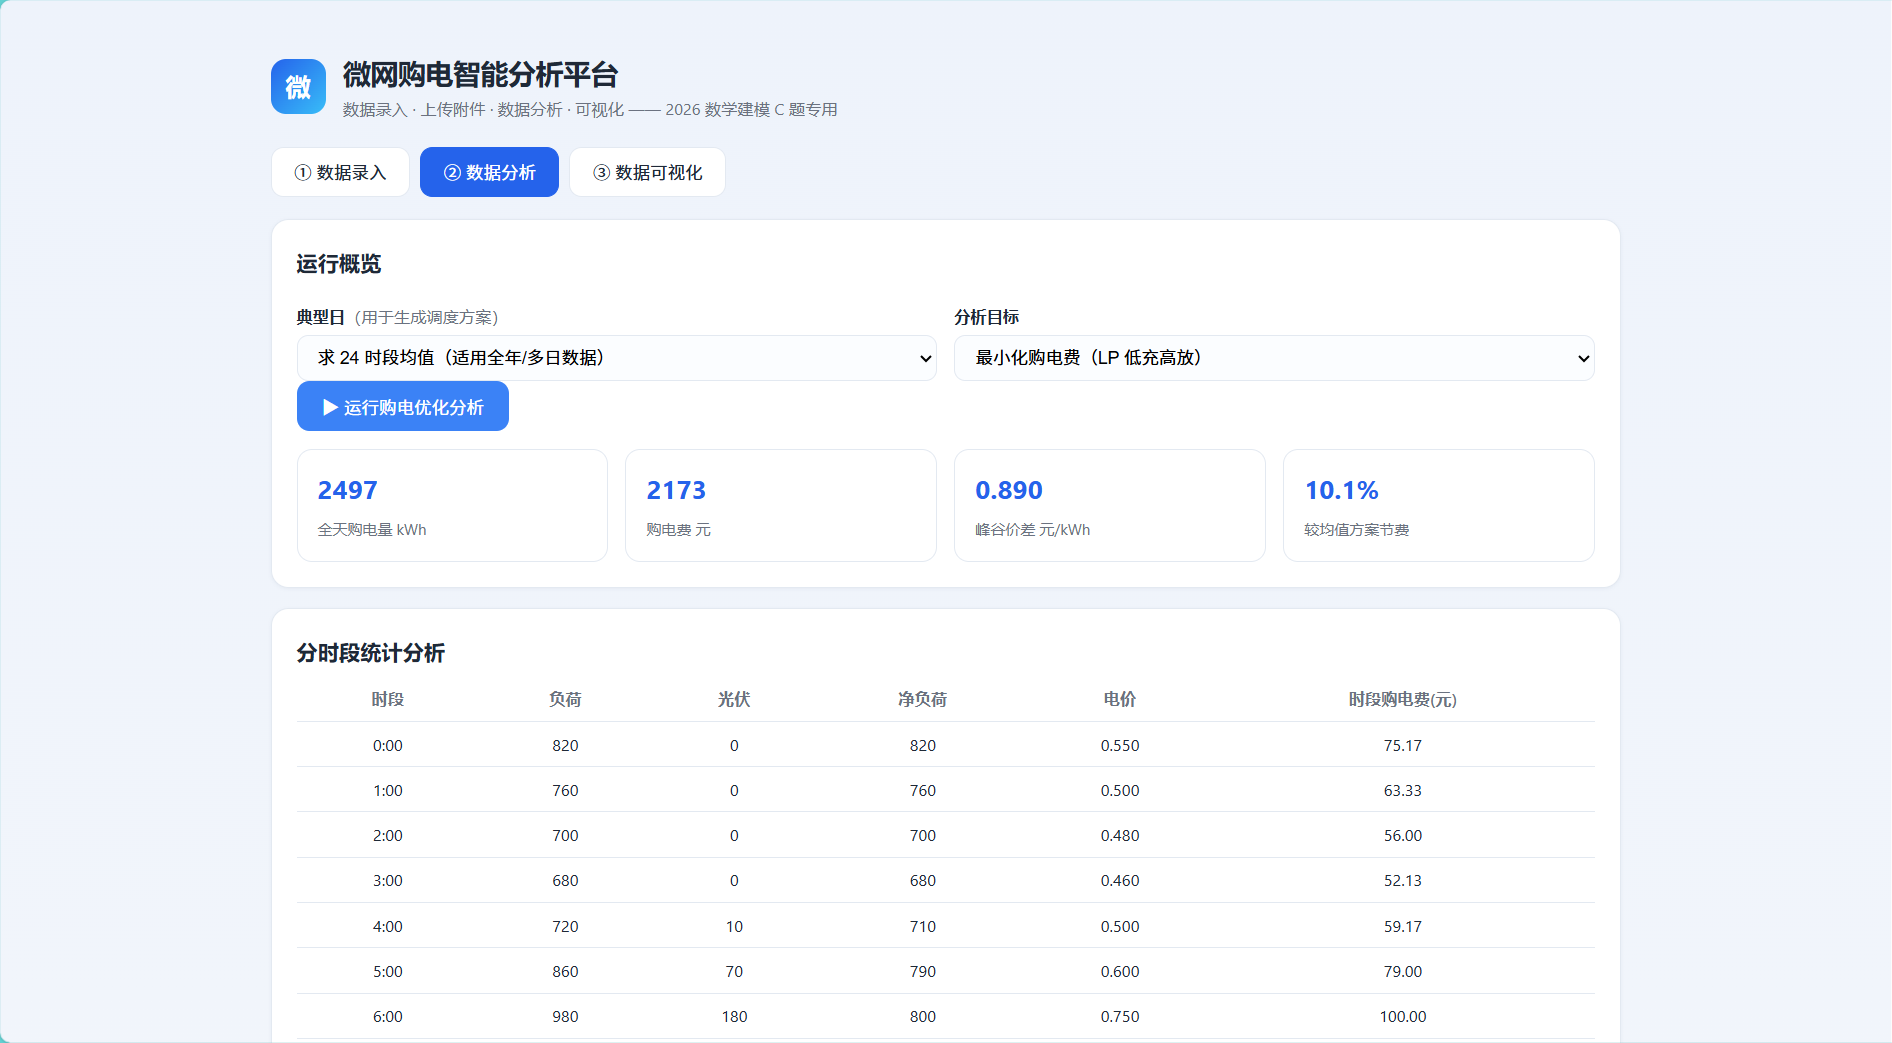
\includegraphics[width=\textwidth]{figures_adv/platform_analysis.png}
    \end{minipage}\hfill
    \begin{minipage}[t]{0.32\textwidth}
        \centering
        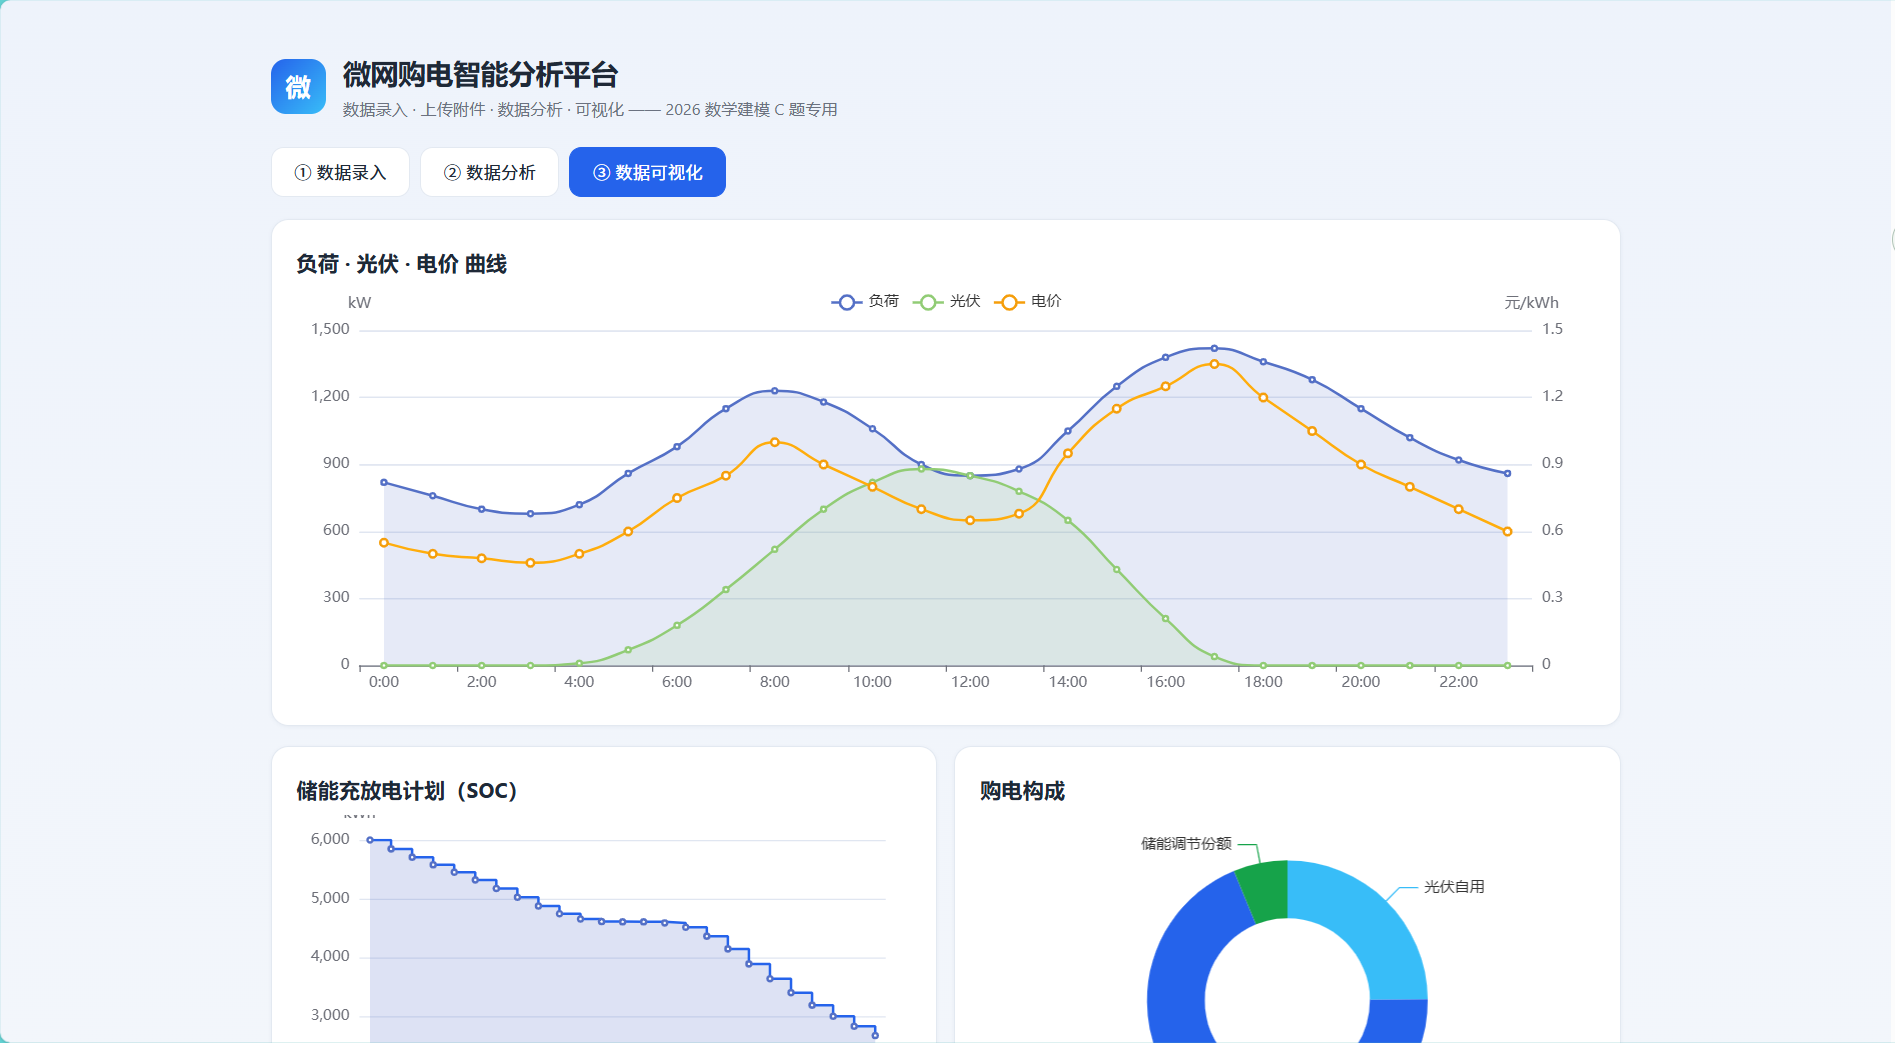
\includegraphics[width=\textwidth]{figures_adv/platform_vis.png}
    \end{minipage}
    \caption{微网购电智能分析平台：数据录入（左）、数据分析（中）、数据可视化（右）}\label{fig:platform}
\end{figure}

\section*{AI 工具使用说明}
本参赛队在竞赛过程中使用了 AI 工具，主要用于语言润色、代码编写与调试、数值结果比对与
排版辅助；核心建模思路、算法设计、模型求解与结果分析均由参赛队自主完成，并对 AI 参与的
内容逐项人工审查与核实。详细使用情况见支撑材料《AI 工具使用详情.pdf》。

\begin{thebibliography}{12}
    \bibitem[1]{cn:microgrid}
    杨苹，许志荣，吴迪，等.
    \newblock 微电网经济调度的研究现状与展望[J].
    \newblock 电力系统自动化，2015，39(16): 108--118.
    \bibitem[2]{cn:microgrid2}
    王成山，李鹏.
    \newblock 分布式发电、微网与智能配电网的发展与挑战[J].
    \newblock 电力系统自动化，2010，34(2): 10--14.
    \bibitem[3]{cn:energy}
    周任军，姚龙华，董小娇，等.
    \newblock 新能源微电网储能系统多目标优化配置[J].
    \newblock 中国电机工程学报，2018，38(7): 1957--1965.
    \bibitem[4]{cn:forecast}
    康重庆，夏清，张伯明.
    \newblock 电力系统负荷预测研究综述与发展方向的探讨[J].
    \newblock 电力系统自动化，2004，28(17): 1--11.
    \bibitem[5]{rp:linprog}
    Huangfu Q., Hall J.
    \newblock Parallelizing the dual revised simplex method[J].
    \newblock Mathematical Programming Computation, 2018, 10(1): 119--142.
    \bibitem[6]{rp:cvar}
    Rockafellar R.T., Uryasev S.
    \newblock Optimization of conditional value-at-risk[J].
    \newblock Journal of Risk, 2000, 2(3): 21--41.
    \bibitem[7]{cn:cvar}
    王守相，王亚昊，刘岩，等.
    \newblock 计及条件风险价值的微电网两阶段随机优化调度[J].
    \newblock 电网技术，2019，43(2): 636--644.
    \bibitem[8]{cn:stoch}
    刘宝碇，赵瑞清.
    \newblock 不确定规划及应用[M].
    \newblock 北京：清华大学出版社，2003.
    \bibitem[9]{cn:mpc2}
    席裕庚.
    \newblock 预测控制[M].
    \newblock 北京：国防工业出版社，2013.
    \bibitem[10]{cn:mpc}
    张旭东，穆钢，严干贵，等.
    \newblock 基于模型预测控制的微网优化调度方法[J].
    \newblock 电工技术学报，2020，35(增刊 1): 26--34.
\end{thebibliography}

\begin{appendices}

\section{支撑材料文件列表}
\begin{itemize}
    \item \texttt{code/}：完整可运行的 Python 源程序（数据加载、LP 求解、情景生成、结果
          写出与绘图，逐问对应 \texttt{main\_q1}~$\sim$~\texttt{main\_q4.py}）；
    \item \texttt{results/}：\texttt{result1}~$\sim$~\texttt{result4} 结果文件（对应附件 5 模板）；
    \item \texttt{figures/}：论文所用图 \texttt{q1\_plan}~$\sim$~\texttt{q4\_price.png}；
    \item \texttt{figures\_adv/}：季节分型、风险敏感性、滚动对比与全年费用结构等分析图（图 A1--A12）；
    \item \texttt{结果说明.md}：结果汇总说明。
\end{itemize}

\section{源程序}
本附录收录建模所用到的全部 Python 源程序（对应支撑材料 \texttt{code/}，共 16 个脚本、约
1433 行）。每个脚本前附一句功能介绍；代码均带行号、等宽缩进，可在 XeLaTeX 下编译并正常
显示中文注释。各脚本按"配置 $\rightarrow$ 数据 $\rightarrow$ 求解器 $\rightarrow$ 情景 $\rightarrow$ 四问入口
$\rightarrow$ 结果回填 $\rightarrow$ 分析 $\rightarrow$ 工具"顺序排列，均可独立运行（需满足 \texttt{config.py} 中的
路径要求）。

\subsection{B.1 全局配置（config.py）}\label{app:config}
确定所有路径、储能参数、电价倍率、时间离散与随机规划参数，供其余脚本统一引用。
\lstinputlisting[language=Python]{../code/config.py}

\subsection{B.2 数据加载与预处理（data.py）}\label{app:data}
读取附件 1--4 全年数据、对齐日期、统一单位为 kWh/时段，并开放各问所需的日矩阵与预报接口。
\lstinputlisting[language=Python]{../code/data.py}

\subsection{B.3 核心求解器（lp.py）}\label{app:lp}
实现单日确定性 LP、固定购电量结算、时段内滚动调整、两阶段随机规划（含 CVaR），
是四问共同依赖的能量守恒 + 储能递推的统一求解内核。
\lstinputlisting[language=Python]{../code/lp.py}

\subsection{B.4 情景生成（scenarios.py）}\label{app:scen}
基于历史残差的非参数 bootstrap，生成点预报与 $S$ 个等概率负荷/光伏情景，供两阶段随机规划使用。
\lstinputlisting[language=Python]{../code/scenarios.py}

\subsection{B.5 问题一入口（main\_q1.py）}\label{app:q1}
单日确定性完美信息；调用 \texttt{solve\_day} 求第 1 问计划购电、充放电与储电轨迹，写出 \texttt{result1.xlsx}。
\lstinputlisting[language=Python]{../code/main_q1.py}

\subsection{B.6 问题二入口（main\_q2.py）}\label{app:q2}
按"完美信息 + 滚动"双口径评估两阶段随机 / CVaR 策略，输出 \texttt{result2.xlsx} 与风险敏感性结果。
\lstinputlisting[language=Python]{../code/main_q2.py}

\subsection{B.7 问题三入口（main\_q3.py）}\label{app:q3}
滚动随机模型预测控制：0:00 计划、6/12/18 调整、实际光伏结算与违约/超额惩罚，写出 \texttt{result3.xlsx}。
\lstinputlisting[language=Python]{../code/main_q3.py}

\subsection{B.8 问题四入口（main\_q4.py）}\label{app:q4}
基于附件 4 波动电价重算问题二、三，输出 \texttt{result4-2.xlsx} / \texttt{result4-3.xlsx} 并做季节对比。
\lstinputlisting[language=Python]{../code/main_q4.py}

\subsection{B.9 结果模板回填（results.py）}\label{app:results}
按附件 5 模板结构用 openpyxl 将计划/调整购电、充放电、紧急购电与储电量写入结果 Excel。
\lstinputlisting[language=Python]{../code/results.py}

\subsection{B.10 季节费用拆分（season\_split.py）}\label{app:season}
固定/波动电价 × 季节的四类日费用真实计算，验证电价波动风险的季节差异。
\lstinputlisting[language=Python]{../code/season_split.py}

\subsection{B.11 季节特征分析（seasonal\_check.py）}\label{app:seasoncheck}
对负荷、光伏与电价做季节分组与统计，支撑问题分析中的季节分型与 ANOVA 检验。
\lstinputlisting[language=Python]{../code/seasonal_check.py}

\subsection{B.12 进阶图表（chart\_advanced.py）}\label{app:chartadv}
生成箱线图、小提琴图、相关热图、帕累托前沿、雷达图、QQ 图、桑基图等分析图（图 A1--A8）。
\lstinputlisting[language=Python]{../code/chart_advanced.py}

\subsection{B.13 问题四图表（chart\_4\_0.py）}\label{app:chart40}
生成风险敏感性、季节费用对比、滚动调整对比与全年费用结构图（图 A9--A12）。
\lstinputlisting[language=Python]{../code/chart_4_0.py}

\subsection{B.14 论文化取数（extract\_paper\_day.py）}\label{app:exday}
从求解结果提取论文正文所需的指定日数值与图数据。
\lstinputlisting[language=Python]{../code/extract_paper_day.py}

\subsection{B.15 论文化取数（extract\_paper\_nums.py）}\label{app:exnums}
汇总全年成本、误差等关键数值，供论文定量表述使用。
\lstinputlisting[language=Python]{../code/extract_paper_nums.py}

\subsection{B.16 页数校验工具（page\_check.py）}\label{app:pagecheck}
统计编译后 PDF 页数，辅助核验"正文 $\le 30$ 页"等篇幅要求。
\lstinputlisting[language=Python]{../code/page_check.py}

\end{appendices}

\end{document}